% Tracing the Consequences of Quantization in Closed-Loop Agents -- ARR October 2026 (NAACL), review version.
% Rewritten 2026-09-30 (RESEARCH_LOG W33) from the retired "perturbation equivalence" draft
% (kept in sections/old/). Binding sources and the provenance of every number: paper/latex/REWRITE_NOTES.md.
% All fork results are \pending{} placeholders until the development and confirmation runs are analysed.
\documentclass[11pt]{article}

\usepackage[review]{acl}

\usepackage{times}
\usepackage{latexsym}
\usepackage[T1]{fontenc}
\usepackage[utf8]{inputenc}
\usepackage{microtype}
\usepackage{inconsolata}
\usepackage{graphicx}
\usepackage{amsmath}
\usepackage{amssymb}
\usepackage{booktabs}
\usepackage{multirow}
\usepackage{xcolor}
\usepackage{xurl}
\usepackage{enumitem}
\usepackage{tikz}
\usetikzlibrary{positioning,arrows.meta,fit}

% ---------------------------------------------------------------------------
% Placeholders for results that do not exist yet. Every \pending{...} names the
% script or output that will fill it and must be resolved before submission.
\newcommand{\pending}[1]{\textcolor{orange}{[PENDING: #1]}}
% Notation
\newcommand{\tautwo}{$\tau^2$-bench}
\newcommand{\pp}{\,pp}
\newcommand{\LL}[1]{L_{\mathrm{#1}}}
\newcommand{\YY}[1]{Y_{\mathrm{#1}}}
\newcommand{\Gall}{G_{\mathrm{all}}}
% ---------------------------------------------------------------------------

\title{Tracing the Consequences of Quantization in Closed-Loop Agents}

\author{Anonymous ARR submission}

\begin{document}
\maketitle

\begin{abstract}
Compressed LLM agents are usually judged against a single run of the full-precision model. We argue that in closed-loop evaluation under greedy decoding this comparison is ill-posed. Composing a published per-step margin model of greedy token flips over an episode, we predict, and observe on Qwen3-4B (consistently on Qwen3-8B), that every perturbation whose logit shifts reach the bf16 grid step (0.125 nats) meets a per-decision divergence floor set by near-ties in free-text turns: a prompt nonce, a compiler kernel choice and 8-bit rounding all re-roll the trajectory. We therefore propose \emph{perturbation equivalence}: a compressed agent is judged by task-level exchangeability with outcomes from the reference model's own perturbation null. On \tautwo{} retail and airline (85 tasks), serving numerics alone move the canonical Qwen3 score by 6--8 points and flip about a quarter of task outcomes, and a single-draw 12-point calibration gain reverses sign on replication. On Qwen3-4B, success is not distinguishable from the null up to the RTN-W4 error scale and drops only near 3 bits, a tentative later damage threshold. \pending{five-model summary sentence --- cells \nolinkurl{a6k2_{q4,q8,q14,q30a3,q32}_*}, scripts \nolinkurl{analysis/insights/iter_1/verify/v01_legacy_recompute.py} a6k2, \nolinkurl{v03_outcomes_pooled.py} a6k2, \nolinkurl{v04_pooled_draws.py}} We close with an evaluator checklist.
\end{abstract}

\section{Introduction}
\label{sec:intro}

Quantized LLM agents are usually compared with their full-precision reference by average task success, and in closed-loop benchmarks such as \tautwo{} \citep{barres2025tau2} that comparison can look reassuring. On our checkpoints, quantized-minus-BF16 success ranges from $-0.2$ to $+4.2$\pp{} across four W4 cells, with new-task (crossed) intervals about $\pm$6--7\pp{} wide (Appendix~\ref{app:e2e}). % src: analysis/insights/iter_4/out/success_ni_ALIGNED_20260930T213009Z.md
Yet the quantized agent (Q) still takes actions that its BF16 reference (B) would not. If B is available as a fallback, as in dynamic precision routing \citep{li2026dynamicmp}, every such state poses a decision: \textbf{upgrade precision for this step only, from the next step on, or both?} In a closed-loop agent, the value of such an upgrade is jointly determined by the action it changes and by the execution that follows.

\paragraph{Judging the two actions is not enough.} Consider a state from our data (q4 AWQ-W4, \tautwo{} airline task 31, nonce block f13, decision 1 of 12). Q looks up a reservation id that does not exist and receives ``not found''; B looks up the user's profile. B's action plainly looks better. We froze this state and ran all four combinations of \{B's or Q's action\} $\times$ \{B or Q continuing\}. Only one succeeds: B's action \emph{followed by} B. If B supplies only this step and Q continues, Q searches for flights, writes a change and fails. If Q's failed lookup stands and B continues, B also fails. % src: analysis/fork/out/ghf_20261001T211519Z.md (§4 Case 5)
At this state, the better-looking action has task value under one continuation and none under the other; judging the action alone cannot reveal this.

\paragraph{A crossed same-state intervention.} At a frozen state whose no-op replay is bit-exact, we cross the source of the current action with the controller of the remaining episode (Figure~\ref{fig:fork}). This turns ``this step'' ($G$), ``from the next step'' ($H$) and ``both'' ($F$) into directly comparable interventions on the same states (\S\ref{sec:method}). The $2\times2$ crossing is a standard factorial design. We study Qwen3-4B and Qwen3-8B (simulated weight and KV-cache quantization, BF16 compute) in \tautwo{} with one greedy user simulator, BFCL multi-turn and ALFWorld, forking at the first decision where the two models' actions differ in tool structure (text-only differences are skipped) and at ordinary states drawn independently of any outcome. % nocheck: design label and model sizes

\paragraph{What we find.}
\begin{itemize}[leftmargin=*,itemsep=1pt,topsep=2pt]
\item \textbf{The value of an action depends on the controller that continues} (\S\ref{sec:r2}). In 26.9\% of development W4 divergent states, the same action swap has a different outcome effect under B's continuation than under Q's. The two effects agree more than a marginal-preserving pairing control expects (38.0\%, $\kappa=0.29$); strict reversals are rare. Post hoc, it also appears on BFCL (4.7--17.1\% per W4 cell) and q8 ALFWorld (32.8--40.0\%), which have no LLM user, and on the telecom holdout (20.7\%). Without a same-precision perturbation control, these shares include the continuation's sensitivity to any change of controller. Cross-cell comparisons are descriptive, and no $G-H$ ordering is established as transferable. % src: analysis/fork/out/ghf_20261001T211519Z.md (§2); analysis/fork/out/agreement_control_20261002T024240Z.md (§2); analysis/fork/out/ext_r2_20261002T024433Z.md (§3); analysis/fork/out/holdout_r2_posthoc_20261002T024414Z.md (§3 pool)
\item \textbf{Local precision upgrades redistribute success and failure} (\S\ref{sec:r1}, \S\ref{sec:r3}). Replacing a W4 agent's first tool-structure-divergent action rescues or damages 15.5--20.9\% of task$\times$block units, while the net effect is $-1.9$ to $+2.9$\pp{}. On 34 pre-registered unseen telecom tasks, the swap again rescues and damages, task fragility repeats, and the estimated effect is $-4.6$\pp{} (90\% CI $-7.2$ to $-2.0$; the frozen primary reading is inconclusive). A local precision patch therefore needs a direct evaluation of its execution consequences. % src: analysis/fork/out/dev_all_20261001T070326Z.md; analysis/fork/out/holdout_confirm_20261002T012353Z.md
\item \textbf{Finding sensitive decisions and choosing beneficial replacements are different learning targets} (\S\ref{sec:r4}). A frozen Q-uncertainty trigger captures more outcome-changing decisions than random selection at two of three rates on later nonce blocks, but has not been shown to select net-beneficial replacements; a hindsight oracle with the same per-cell budget nets $+3.3$ to $+3.7$\pp{}. Mixed-precision selection thus has to predict rescues and damages jointly, not divergence alone. % src: analysis/fork/out/token_mech_20261002T003130Z.md (§3); analysis/fork/out/oracle_trigger_20261002T024423Z.md (§1a)
\end{itemize}

\paragraph{Contributions.} (1)~A crossed-intervention evaluation framework for precision upgrades in agents: same-state restoration with bit-exact replay acceptance, full-action interventions, paired estimands ($G$, $H$, $F$ and the $(\DQ,\DB)$ table) with explicit denominators, and inference that separates a fixed task pool from new tasks. (2)~Systematic findings over weight, KV-cache and stress quantization, two model sizes and three benchmarks: two-sided consequences, controller dependence across environments, text actions at ordinary states (labels not reproduced under a second simulator; \S\ref{sec:r3}) and diagnostics for precision selection. Withdrawn results are in Appendix~\ref{app:withdrawn}. % nocheck: list labels (1)-(2)

Evaluating a precision upgrade for an agent thus requires measuring the task value of the replacement under the execution that follows it, rather than the replaced action in isolation or either model's average success.

\begin{figure}[t]
\centering
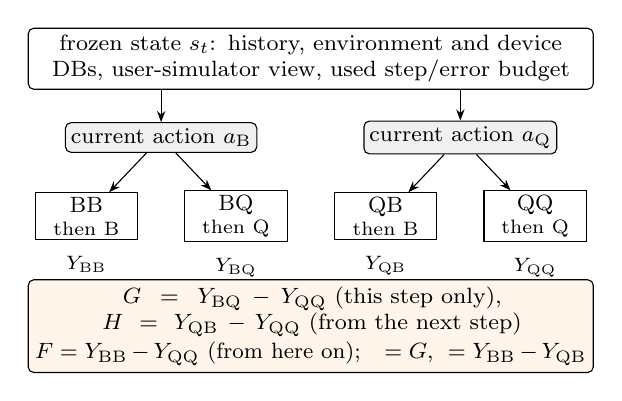
\begin{tikzpicture}[ % nocheck: TikZ layout coordinates
  font=\footnotesize,
  box/.style={draw, rounded corners=2pt, align=center, inner sep=2.5pt},
  act/.style={draw, rounded corners=2pt, align=center, inner sep=2pt, fill=gray!12}, % nocheck: TikZ style
  br/.style={draw, align=center, inner sep=1.5pt, minimum width=1.3cm},
  arr/.style={-{Stealth[length=4pt]}, thin}]
\node[box, text width=7.0cm] (h) at (0,0) {frozen state $s_t$: history, environment and device DBs, user-simulator view, used step/error budget}; % nocheck: TikZ
\node[act] (aB) at (-1.9,-1.0) {current action $a_{\mathrm{B}}$}; % nocheck: TikZ
\node[act] (aQ) at (1.9,-1.0) {current action $a_{\mathrm{Q}}$}; % nocheck: TikZ
\draw[arr] (h.south -| aB) -- (aB); \draw[arr] (h.south -| aQ) -- (aQ);
\node[br] (bb) at (-2.85,-2.0) {BB\\[-1pt]{\scriptsize then B}}; % nocheck: TikZ
\node[br] (bq) at (-0.95,-2.0) {BQ\\[-1pt]{\scriptsize then Q}}; % nocheck: TikZ
\node[br] (qb) at (0.95,-2.0) {QB\\[-1pt]{\scriptsize then B}}; % nocheck: TikZ
\node[br] (qq) at (2.85,-2.0) {QQ\\[-1pt]{\scriptsize then Q}}; % nocheck: TikZ
\draw[arr] (aB) -- (bb); \draw[arr] (aB) -- (bq);
\draw[arr] (aQ) -- (qb); \draw[arr] (aQ) -- (qq);
\foreach \n/\l in {bb/BB,bq/BQ,qb/QB,qq/QQ} {\node[below=0.08cm of \n, font=\scriptsize] (y\n) {$Y_{\mathrm{\l}}$};} % nocheck: TikZ
\node[box, text width=7.0cm, fill=orange!8, anchor=north] (cat) at (0,-2.8) % nocheck: TikZ
  {$G=\YY{BQ}-\YY{QQ}$ (this step only),\; $H=\YY{QB}-\YY{QQ}$ (from the next step)\\[1pt]
   $F=\YY{BB}-\YY{QQ}$ (from here on);\quad $\DQ=G$,\; $\DB=\YY{BB}-\YY{QB}$};
\end{tikzpicture}
\caption{Crossed same-state intervention (schematic, not data). B = BF16 agent, Q = quantized agent. In branch XY, the first letter is the source of the current action and the second is the controller from the next step to the end. Every branch starts from the same frozen state with the original remaining budget. QQ re-executes Q's original episode, and its bit-exact reproduction is the no-op check. Definitions are in \S\ref{sec:estimands}.}
\label{fig:fork}
\end{figure}

\section{Related Work}
\label{sec:related}

\paragraph{Episode-level comparisons of quantized agents.} \emph{Flat Score, Amplified Failures} \citep{jang2026flat} is the closest study in setting. On \tautwo{} retail and telecom it shows that 4-bit agents keep a flat task score while process damage grows. It reports a two-sided paired task split (33 tasks worse, 26 better for Gemma-4-31B on telecom) and explains the flat score by the error budget and by recovery, equally frequent at both precisions (55\% after a failed call). % src: docs/insights/FLATSCORE_COMPARISON.md
Its comparisons are between independently sampled episodes, so the precision of the action that went wrong and the precision of the controller that must recover change together. Our design holds the state fixed and varies the two separately. $H$ measures what the recovering controller contributes on identical histories, and the $(\DQ,\DB)$ table measures whether an action's consequence depends on that controller. Two-sided flips under compression were first shown on static tasks \citep{dutta2024accuracy}; agent-compression benchmarks report averages \citep{dong2025acbench}.

\paragraph{Live forks with a model switch.} \emph{The Replay Gap} \citep{gonuguntla2026replay} forks live SWE-agent trajectories at a fixed step and continues them with a different model (Qwen3-4B FP8 vs.\ Qwen3-14B AWQ), against same-model control forks. At the switch point the new model produces the next action \emph{and} the continuation, so the two change together; this is our $F$ contrast, not $G$ or $H$. Its 359 control forks had 0 success flips; we claim no noise advantage. % src: outputs/.drafts/storyline-v7-lit.md (row 1) Single-step action swaps under a fixed continuation fill one cell of our design and are used for training \citep{li2026cso,li2026crr}, attribution \citep{shah2026car} and locating decisive errors \citep{zhang2025agentracer}. None of the 32 closest works we checked crosses the action with the continuation controller at a precision-induced divergence. % src: outputs/.drafts/storyline-v7-lit.md (TL;DR, findings (b))

\paragraph{Precision routing and its proxies.} DMR \citep{li2026dynamicmp} learns a per-step BF16/W4 router from BF16-versus-quantized KL supervision and episode reward. Precision sensitivity has also been localised to phases \citep{lu2026mixquant} and task types \citep{zhang2026quantclaw}. We do not propose a competing router. We measure what a router would harvest, namely the intervention gains $G$, $H$ and $F$ at given states, and we test whether a Q-visible proxy predicts them. For quantized reasoning models, \citet{lotfi2026quantized} trace damage to high-entropy, high-KL token positions where markers such as ``wait'' are over-sampled; \S\ref{sec:r4} tests the analogue for agent actions.

\paragraph{Evaluation noise and user simulators.} Prefix caching changed multi-turn tool-use trajectories in 36.2\% of episodes at 16-bit and 75.0\% at 4-bit \citep{patodiya2026same}; agentic evaluations vary from run to run \citep{bjarnason2026randomness,chen2026noisefloor}, and with the user model (\S\ref{sec:r3}). % src: outputs/.drafts/storyline-v7-lit.md (row 16)

\section{Run Conditions and Measurement Definitions}
\label{sec:conditions}

\paragraph{Tasks.} We use \tautwo{} \citep{barres2025tau2} in text mode. \emph{Development} uses the 85 retail and airline tasks of our frozen evaluation split (58 retail, 27 airline; 22 tasks were excluded earlier because BF16 was unstable on them, and they stay out because that selection used BF16 behaviour) and the 80-task telecom development split. \emph{Confirmation} uses the remaining 34 telecom tasks. The telecom split was fixed before any run from \tautwo{}'s official 114-task \texttt{base} split, stratified by issue type and persona and ordered by a salted hash of the task id, so no model output entered it. A disjoint set of 57 retail/airline tasks supplies the quantizers' calibration trajectories.

\paragraph{Agents and quantization.} The agents are Qwen3-4B-Instruct-2507 (q4) and Qwen3-8B (q8, thinking disabled), pinned to fixed revisions and served with the Hermes tool parser. The user simulator is Qwen3-30B-A3B, shared by all agents. Q is a GPTQ-W4 \citep{frantar2023gptq} or AWQ-W4 \citep{lin2024awq} checkpoint, fake-quantized: weights are quantized and dequantized, then served with BF16 compute on the same serving path as the BF16 reference B. The primary checkpoint per model and method (calibration draw d1) was fixed by a completeness rule stated before any fork outcome (the checkpoint with the most existing independent runs; ties broken by the lowest draw index), not by earlier results. Agent and simulator decode greedily with a 32k-token context.

\paragraph{Deterministic serving.} Agents and simulator run on vLLM with batch-invariant kernels and deterministic Inductor compilation; every server start checks a numerics canary against stored reference outputs. We adopted the deterministic compilation flag after finding that compile-time autotuning chose different reduction configurations for a fused residual+RMSNorm kernel on different nodes, which shifted every token of a determinism pair (Appendix~\ref{app:serving}). With the fix, cross-node determinism pairs are byte-identical in prompts and completions: 257/257 decisions for q4 and 303/303 for Qwen3-30B-A3B as agent. Each branch of \S\ref{sec:fork} is therefore designed to have one reproducible outcome given its state; the replay acceptance gate (\S\ref{sec:replay}) checks this rather than assuming it.

\paragraph{Prompt nonces and blocks.} A \emph{nonce} is a short random string inserted as a session-identifier line in the system prompt. It is a researcher-defined input perturbation, not a ``no-change'' null: it changes the input and re-rolls trajectories. We use it for one purpose: each independent nonce defines a \emph{block}, one closed-loop run of Q (and of B, for paired success) over the task pool, and blocks are the replicate unit of inference (\S\ref{sec:inference}). Reference controls are reported separately and never pooled with the quantization comparison: identical-setting repeats, nonce perturbation, numerics controls (a rotated-BF16 checkpoint) and fixed random weight perturbations, the last being a control intervention rather than a null. \pending{stratified floor table for these controls, flagging single canonical-run floors --- identical-setting repeats and a BF16-vs-BF16 nonce control are not run yet (\nolinkurl{docs/insights/METHODOLOGY_REVISION.md} B4)}

\paragraph{Success endpoints.} For retail and airline we report \emph{DB success}: the final database matches the gold database and the episode terminated normally. This is not \tautwo{}'s official reward, which multiplies DB match with natural-language assertions (retail, 112 of 114 tasks) or a communicate check (airline, 50 of 50); official rewards are reported separately. For telecom we report the official deterministic task-basis success (environment assertions, plus action checks for 14 of the 80 development tasks). Context overflow and unparseable agent output count as failures; infrastructure outages are missing, never failures, and never ``no divergence''.

\paragraph{Tool types.} Whether an action reads, writes or hands off is taken from a table derived from \tautwo{}'s tool decorators and re-verified against the source (Table~\ref{tab:tooltypes}); names outside a domain's tool list are \emph{invalid}. An earlier name-pattern rule agreed with the table on 99.98\% of q4/q8 episodes for ``any write'' in retail/airline, but misses 5 of the 6 telecom write tools, so the table is binding for all annotation and is frozen by hash before confirmation.

\begin{table}[t]
\centering\footnotesize\setlength{\tabcolsep}{4pt}
\resizebox{\columnwidth}{!}{\begin{tabular}{@{}lccccc@{}}
\toprule
Domain & read & write & handoff & other & regex misses \\
\midrule
Retail  & 7 & 7 & 1 & 1 (calculate) & 0 \\
Airline & 6 & 6 & 1 & 1 (calculate) & 0 \\
Telecom & 6 & 6 & 1 & 0 & 5 of 6 writes \\
\bottomrule
\end{tabular}}
\caption{Agent tool types per domain, from the \tautwo{} tool decorators (commit \texttt{2174a60}), verified by re-derivation from the source. ``Regex misses'': write tools the earlier name-pattern rule failed to classify. Source: \nolinkurl{analysis/insights/iter_4/out/tool_types.json}; full list in Appendix~\ref{app:tooltable}.}
\label{tab:tooltypes}
\end{table}

\paragraph{Background measurement: turnover above a floor.} As motivation only, and only for the conditions where it was verified (5 Qwen3 models, retail and airline, W4 cells against a numerics floor of rotated BF16, canonical BF16 reruns and Gaussian noise at $k\le 0.003$), the turnover intensity of W4 checkpoints exceeds the floor: pooled excess $+0.19$ [0.10, 0.30] for RTN, $+0.15$ for GPTQ and $+0.16$ for AWQ, Holm-adjusted (Appendix~\ref{app:turnover}). This says that W4 changes which tasks succeed. It does not say which of those changes quantized actions cause, which is the question of \S\ref{sec:fork}. Whether W4 success is non-inferior to BF16 is a separate, paired analysis (margin 3\pp{}; \S\ref{sec:confirm}). \pending{paired Q$-$B success non-inferiority, TOST and ordinary difference per model $\times$ method --- \nolinkurl{analysis/insights/iter_4/success_ni.py} real mode on the \nolinkurl{a6k2_{q4,q8}_bfpair_q1..q5} runs}

\section{Same-State Four-Branch Design}
\label{sec:fork}

\subsection{Fork states: the first semantic action divergence}
\label{sec:states}

For a model, a quantized checkpoint Q, a task $i$ and a block $r$, take Q's closed-loop trajectory. Before each of Q's decisions $t$ we restore the saved state $s_t$: the full message history (agent, user and tool messages), the environment and user-device databases rebuilt by strict replay of the recorded tool calls, the user simulator's visible conversation, and the step and error budget already used. B then generates its full action on the same request; the prompt token ids B's server receives must equal those Q received at $t$, otherwise the task is excluded with that reason. The primary state is the first $t$ at which the two full actions differ \emph{semantically}: in class (tool call, text, stop), in tool name (including names outside the domain's tool list), in the number or order of calls, or in arguments after normalisation (key order, JSON whitespace and number formatting ignored).
\begin{itemize}[leftmargin=*,itemsep=1pt,topsep=2pt]
\item At most one state per task $\times$ model $\times$ checkpoint $\times$ block, frozen (written to disk with its hashes) before any branch is run.
\item Differences in free text only (same class, different wording) are recorded but are not primary states. Such differences, for example a commitment made or an authorisation requested in prose, can matter; they are outside the primary scope.
\item Late divergences are kept, with their remaining step and error budget.
\item A task with no qualifying divergence stays in the denominator with zero effect. Infrastructure failures are never coded as ``no divergence''.
\end{itemize}

\subsection{Branches and estimands}
\label{sec:estimands}

From state $s$, the current action $a_{\mathrm{X}}$ ($\mathrm{X}\in\{\mathrm{B},\mathrm{Q}\}$) is executed as the agent's next step by the real environment or answered by the real simulator, consuming one step and counting its errors as in live play; controller $\mathrm{Y}$ then continues to the end with the original remaining budget. This gives branches BB, BQ, QB and QQ with binary outcomes $\YY{XY}$ and means $\LL{XY}=E[\YY{XY}]$ over fork states (Figure~\ref{fig:fork}). QQ reproduces Q's original episode.

\paragraph{One-replacement gain.} Replacing only the current action with B's, while Q continues, gives
\begin{equation}
G = E[\YY{BQ}-\YY{QQ}] = h - b,
\end{equation}
with rescue rate $h=P(\YY{BQ}=1,\YY{QQ}=0)$ and new-damage rate $b=P(\YY{BQ}=0,\YY{QQ}=1)$. We always report the paired four-way composition (rescue, new damage, both succeed, both fail), because the same $G$ can come from few consequences or from many rescues cancelled by many breaks.

\paragraph{Decomposition.} With B's branch BB as the reference,
\begin{align}
A &= \LL{QB}-\LL{BB} \quad\text{(current action)},\\
C &= \LL{BQ}-\LL{BB} \quad\text{(continuation)},\\
I &= \LL{QQ}-\LL{QB}-\LL{BQ}+\LL{BB} \quad\text{(interaction)},
\end{align}
so that $\LL{QQ}-\LL{BB}=A+C+I$ exactly, and $G=-(A+I)$: the gain of one replacement is the current-action effect as seen under Q's own continuation. $A$, $C$ and $I$ are contrasts on the population of fork states; they say where the change in success at a divergence comes from, not whether a particular action was wrong (\S\ref{sec:annotation}).

\paragraph{Primary endpoint.} Let $D_{ir}=1$ if task $i$ in block $r$ reaches a valid fork state. The primary endpoint is the full-pool one-replacement gain
\begin{equation}
\Gall = E_{i,r}\big[D_{ir}\,(\YY{BQ}-\YY{QQ})_{ir}\big] = \pi\, G,
\end{equation}
with divergence prevalence $\pi=P(D_{ir}=1)$, averaged over the whole task pool with fixed cell weights declared in advance; tasks without a divergence contribute zero. The conditional $G$ (given a divergence) is secondary and is estimated as a ratio with block resampling. Prevalence, the number of valid states and every exclusion reason are always reported.

\subsection{Replay acceptance}
\label{sec:replay}

Forks count as mechanism evidence only if an engineering gate passes before any development outcome is analysed:
(a) restoration of the databases, device state, user-simulator state and step budget is correct, and canonical state hashes match after save and load;
(b) no-op forks B$\to$B and Q$\to$Q reproduce the original trajectories and outcomes, token for token;
(c) with B and Q pointed at the same checkpoint (on two servers), all four branches agree;
(d) branches are isolated, so execution order and concurrency do not change any branch;
(e) after a controller switch the context is re-prefilled from the history by the other server, with no KV or prefix cache shared across weights; and forced actions consume the same step and error budget as live actions.
If restoration cannot be verified by the decision point, the paper reports the measurements of \S\ref{sec:states} and \S\ref{sec:annotation} and withdraws the causal reading of the branches. \pending{gate outcome (a)--(e) with counts --- \nolinkurl{analysis/fork/gate/} (\nolinkurl{gate.json}, \nolinkurl{gate_same.json}) from \nolinkurl{scripts/a6000/fork_driver.py}; \nolinkurl{docs/insights/FORK_PROTOCOL.md} \S8}

\subsection{Protocol, replicates and inference}
\label{sec:inference}

\paragraph{Deterministic protocol.} Under deterministic serving and a greedy simulator, each branch is run once per state; the randomness in $\Gall$ comes from which states arise, and that varies only across blocks. A block is one independent nonce (\S\ref{sec:conditions}); all tasks of a block share it, and B and Q branches share each state, so inference is on paired blocks: we compute each block's full-pool statistics and draw intervals from between-block variation, with simulation checks of calibration for sparse events. \pending{interval method and its simulated coverage for sparse rescue/damage counts --- statistics deliverable (review \S D), script in \nolinkurl{analysis/fork/} not yet written}

\paragraph{Stochastic fallback.} If deterministic replay fails the gate but the start state (environment, history, remaining budget) is verifiably identical across branches and the remaining differences come from a describable, repeatable source of randomness in the subsequent execution, the estimand becomes $G=E[\YY{BQ}]-E[\YY{QQ}]$, the expectation over that declared randomness. Branch repeats estimate these expectations and are nested within task, nonce and state; they are not independent samples. Same-configuration replays measure run variance but are never subtracted from $G$ as a ``no-op flip rate''. Hidden-state loss, branch contamination or systematic replay bias cannot be repaired by repeats. Repeat count, seed rule, failure handling and inference would be fixed in the protocol before use.

\paragraph{Two target populations.} Conclusions about the \emph{fixed benchmark task pool} treat tasks as fixed and blocks as random; conclusions about a \emph{new task distribution} resample tasks and blocks jointly (task-clustered, crossed). More nonce blocks narrow the first but not the second; only more independent tasks narrow the second. We report both and never let the first stand in for the second.

\paragraph{Decision rules.} We plan power for a true $G$ of $g_{\min}=3$\pp{}. $G$ is called positive if its one-sided 95\% lower bound exceeds 0, and above 3\pp{} if that bound exceeds 3\pp{}. An average effect is called small only if a valid 90\% interval lies inside $(-3,+3)$\pp{}. A 5\pp{} margin is a sensitivity analysis only. A pooled pass does not imply a per-model or per-method pass. \pending{multiplicity rule across models, methods and secondary endpoints --- to be frozen in \nolinkurl{docs/insights/PREREG_FORK_CONFIRM.md}}

\subsection{Development results}
\label{sec:fork-results}

Development covers q4 and q8 $\times$ GPTQ-W4 and AWQ-W4 on the 85 retail/airline tasks and the 80 telecom development tasks. The number of blocks is set by simulator throughput, after the gate, full task coverage and complete, balanced blocks, with capacity reserved for the confirmation (Table~\ref{tab:dev}).

\begin{table*}[t]
\centering\scriptsize\setlength{\tabcolsep}{4pt}
\resizebox{\textwidth}{!}{\begin{tabular}{@{}llccccc@{}}
\toprule
 & Quantity & q4 GPTQ-W4 & q4 AWQ-W4 & q8 GPTQ-W4 & q8 AWQ-W4 & Pooled (fixed weights) \\
\midrule
\multirow{6}{*}{\shortstack[l]{(a) Divergence\\coverage}}
 & tasks in pool $\times$ blocks & \pending{DEV-a} & \pending{DEV-a} & \pending{DEV-a} & \pending{DEV-a} & \pending{DEV-a} \\
 & valid fork states & \pending{DEV-a} & \pending{DEV-a} & \pending{DEV-a} & \pending{DEV-a} & \pending{DEV-a} \\
 & no qualifying divergence & \pending{DEV-a} & \pending{DEV-a} & \pending{DEV-a} & \pending{DEV-a} & \pending{DEV-a} \\
 & excluded (by reason) & \pending{DEV-a} & \pending{DEV-a} & \pending{DEV-a} & \pending{DEV-a} & \pending{DEV-a} \\
 & prevalence $\pi$ [CI] & \pending{DEV-a} & \pending{DEV-a} & \pending{DEV-a} & \pending{DEV-a} & \pending{DEV-a} \\
 & position $t$ / remaining budget (median) & \pending{DEV-a} & \pending{DEV-a} & \pending{DEV-a} & \pending{DEV-a} & \pending{DEV-a} \\
\midrule
\multirow{4}{*}{\shortstack[l]{(b) Consequence\\composition\\$(\YY{BQ},\YY{QQ})$}}
 & rescue $(1,0)$: $n$ (share) & \pending{DEV-b} & \pending{DEV-b} & \pending{DEV-b} & \pending{DEV-b} & \pending{DEV-b} \\
 & new damage $(0,1)$: $n$ (share) & \pending{DEV-b} & \pending{DEV-b} & \pending{DEV-b} & \pending{DEV-b} & \pending{DEV-b} \\
 & both succeed $(1,1)$: $n$ (share) & \pending{DEV-b} & \pending{DEV-b} & \pending{DEV-b} & \pending{DEV-b} & \pending{DEV-b} \\
 & both fail $(0,0)$: $n$ (share) & \pending{DEV-b} & \pending{DEV-b} & \pending{DEV-b} & \pending{DEV-b} & \pending{DEV-b} \\
\midrule
\multirow{6}{*}{\shortstack[l]{(c) Gain and\\decomposition\\(pp, 95\% CI)}}
 & $\Gall$ (primary, fixed pool) & \pending{DEV-c} & \pending{DEV-c} & \pending{DEV-c} & \pending{DEV-c} & \pending{DEV-c} \\
 & $\Gall$ (new tasks) & \pending{DEV-c} & \pending{DEV-c} & \pending{DEV-c} & \pending{DEV-c} & \pending{DEV-c} \\
 & $G$ given divergence & \pending{DEV-c} & \pending{DEV-c} & \pending{DEV-c} & \pending{DEV-c} & \pending{DEV-c} \\
 & $A$ (current action) & \pending{DEV-c} & \pending{DEV-c} & \pending{DEV-c} & \pending{DEV-c} & \pending{DEV-c} \\
 & $C$ (continuation) & \pending{DEV-c} & \pending{DEV-c} & \pending{DEV-c} & \pending{DEV-c} & \pending{DEV-c} \\
 & $I$ (interaction) & \pending{DEV-c} & \pending{DEV-c} & \pending{DEV-c} & \pending{DEV-c} & \pending{DEV-c} \\
\bottomrule
\end{tabular}}
\caption{Development forks (85 retail/airline + 80 telecom development tasks), per model $\times$ method and pooled with fixed cell weights. All cells are placeholders. \pending{DEV-a: coverage from the frozen state files (\nolinkurl{states/*.json}) written by \nolinkurl{scripts/a6000/fork_driver.py}; DEV-b, DEV-c: branch outcomes from \nolinkurl{fork_driver.py} and the paired-block analysis script to be added under \nolinkurl{analysis/fork/}; per-domain split in the appendix}}
\label{tab:dev}
\end{table*}

\section{Consequence Composition and Mechanism Annotation}
\label{sec:annotation}

A different full action is not by itself a mechanism finding, and a nonzero $G$ does not say why. For each fork state and branch we therefore record process evidence in three independent fields. The BF16 action is only a reference: a Q action is never labelled defective because it differs from $a_{\mathrm{B}}$, and $a_{\mathrm{Q}}$ and $a_{\mathrm{B}}$ are judged by the same checks.
\begin{enumerate}[leftmargin=*,itemsep=1pt,topsep=2pt]
\item \textbf{Defect of the current action}, judged from tool preconditions, task requirements, authorisation and state changes: an invalid tool (Table~\ref{tab:tooltypes}), invalid arguments against the tool schema, an execution error returned by the environment, identifiers that appear in no earlier message or tool output, a write without an explicit confirmation in the preceding user turn (a proxy, not an authorisation verdict), a malformed action, or ending the episode.
\item \textbf{Later correction aimed at that defect}, e.g.\ a later valid call of the same tool with grounded identifiers; a write is not undone by a retry.
\item \textbf{Requirements satisfied at the end}: success under its named endpoint, each environment assertion, action and communicate check, and the database paths that differ from the gold state.
\end{enumerate}
Recovery is claimed only for the sequence \emph{defect $\rightarrow$ correction $\rightarrow$ requirements satisfied}. Otherwise a failed branch reads ``not recovered under the tested continuation controllers and the fixed remaining budget''. We also relate non-recovery to the remaining budget, the defect type and the controller.

% Table 4 (holdout) is defined here so that it floats onto the page of Section 6.
\begin{table*}[t]
\centering\scriptsize\setlength{\tabcolsep}{4pt}
\resizebox{\textwidth}{!}{\begin{tabular}{@{}lccccc@{}}
\toprule
Quantity & q4 GPTQ-W4 & q4 AWQ-W4 & q8 GPTQ-W4 & q8 AWQ-W4 & Pooled (fixed weights) \\
\midrule
blocks / valid fork states / no divergence / excluded & \pending{HOLD} & \pending{HOLD} & \pending{HOLD} & \pending{HOLD} & \pending{HOLD} \\
rescue / new damage / both succeed / both fail: $n$ (share) & \pending{HOLD} & \pending{HOLD} & \pending{HOLD} & \pending{HOLD} & \pending{HOLD} \\
$\Gall$ (pp) [one-sided 95\% lower bound] & \pending{HOLD} & \pending{HOLD} & \pending{HOLD} & \pending{HOLD} & \pending{HOLD} \\
$A$, $C$, $I$ (pp) [95\% CI] & \pending{HOLD} & \pending{HOLD} & \pending{HOLD} & \pending{HOLD} & \pending{HOLD} \\
frozen hypothesis: verdict & \multicolumn{5}{c}{\pending{HOLD}} \\
\bottomrule
\end{tabular}}
\caption{Telecom holdout confirmation (34 tasks). All cells are placeholders. \pending{HOLD: holdout fork runs under the frozen \nolinkurl{docs/insights/PREREG_FORK_CONFIRM.md} (not yet written), analysed by the same \nolinkurl{analysis/fork/} script as Table~\ref{tab:dev}}}
\label{tab:confirm}
\end{table*}

\paragraph{Three layers of labels.} (i) \emph{Automatic events} are extracted on all trajectories from the tool-type table, the tool schemas, environment responses and the evaluator, keeping the raw record behind each judgement. (ii) An \emph{LLM labeller} assigns correction and failed-requirement labels under fixed written rules; every label carries its evidence location in the trajectory, and ``cannot judge'' is an allowed answer. Labels such as ``wrong identifier'', ``write without consent'' and ``premature end'' need rule support or human review, because legitimate substitutes, earlier authorisation and already completed tasks exist. (iii) \emph{Blinded human review} covers about 80 fork states, stratified by consequential versus non-consequential pair, tool type and automatic label; about 20 are reviewed independently by two people. Blinding strips model, precision and branch source and randomises order. We report stratified confusion matrices of human against automatic and LLM labels for the key defect and recovery labels; because the sample is enriched, these do not estimate whole-data accuracy. Case studies are drawn only from human-verified states.

\paragraph{Reading $G$ near zero.} The composition and the process fields decide how a small $G$ is read: a wide interval is \emph{inconclusive}; many rescues and many breaks mean \emph{cancellation}; branches that usually both succeed mean a \emph{small consequence}; and an explicit Q defect, then a correction, then success is \emph{observed recovery}.

\begin{table}[t]
\centering\scriptsize\setlength{\tabcolsep}{3pt}
\resizebox{\columnwidth}{!}{\begin{tabular}{@{}lccc@{}}
\toprule
Defect type (current Q action) & states & new damage & recovered \\
\midrule
invalid tool / invalid arguments & \pending{MECH} & \pending{MECH} & \pending{MECH} \\
execution error & \pending{MECH} & \pending{MECH} & \pending{MECH} \\
ungrounded identifier & \pending{MECH} & \pending{MECH} & \pending{MECH} \\
unconfirmed write & \pending{MECH} & \pending{MECH} & \pending{MECH} \\
ends episode & \pending{MECH} & \pending{MECH} & \pending{MECH} \\
no verifiable defect & \pending{MECH} & \pending{MECH} & \pending{MECH} \\
\midrule
human vs.\ auto / LLM agreement & \multicolumn{3}{c}{\pending{MECH-h}} \\
double-review agreement ($\approx$20) & \multicolumn{3}{c}{\pending{MECH-h}} \\
\bottomrule
\end{tabular}}
\caption{Process evidence for development fork states. ``Recovered'' requires defect $\rightarrow$ correction $\rightarrow$ requirements satisfied. \pending{MECH: \nolinkurl{annotations.jsonl} from \nolinkurl{cloq/fork_annotate.py} plus LLM labels (labeller and rules not yet fixed); MECH-h: blinded review sheets and confusion matrices, stratified, in the appendix}}
\label{tab:mech}
\end{table}

\paragraph{Development evidence gate.} There is no go/no-go on the sign of $G$. Development ends when divergence consequences are measured clearly enough to yield a specific explanation that the holdout can test: stable consequences with mechanism evidence; a small effect with a narrow interval and a checked rescue/damage balance; or a few pre-defined divergence types with their opportunity denominators. If intervals are wide and events few, we report insufficient evidence and no new explanation. \pending{which of these outcomes development produced, and the frozen hypothesis for \S\ref{sec:confirm}}

\section{Independent Confirmation}
\label{sec:confirm}

\paragraph{Holdout.} The 34 telecom holdout tasks have not been run by any agent in this study. Telecom differs from retail and airline in its tools and requirements, and in dual control: the user acts on a simulated device, so both sides' tool calls change state. Before the holdout is opened, the mechanism categories found in development are mapped to telecom tools and requirements; the telecom development tasks may be used to debug the tool table and to check that the categories fit, with every rule change logged. The protocol, the tool-type table (by hash), the hypothesis, the number of blocks and the stopping rule are then frozen in a pre-registration file. The block count is derived from the development block variance, not fixed in advance.

\paragraph{Thresholds and their rationale.} The confirmation uses the thresholds of \S\ref{sec:inference}: $g_{\min}=3$\pp{} for $G$, and, for the background success comparison, a non-inferiority margin $\varepsilon=3$\pp{} (H$_0$: success$_{\mathrm{Q}}-$success$_{\mathrm{B}}\le-\varepsilon$; pass if the one-sided 95\% lower bound exceeds $-3$\pp{}). The margin was written down before any paired BF16 outcome existed. On the 85-task pool, 3\pp{} is a change of about 2.5 task outcomes per run. The run-level nonce SD of one checkpoint was 2.5\pp{} on q4 and 2.9\pp{} on q8, so a smaller margin could not be reached with a few paired blocks; a 5\pp{} margin would sit at the size of the largest W4 checkpoint effect we observed (q8 AWQ-W4 d3, $+5.3$\pp{} on average), so it could not flag such a checkpoint. Using one margin for $G$ and for success keeps ``negligible'' consistent. Non-inferiority is not equivalence: equivalence additionally needs the two one-sided tests, with the 90\% interval inside $(-3,+3)$\pp{}, and a margin the data cannot resolve is reported as inconclusive.

\paragraph{What counts as confirmation.} The frozen development hypothesis is tested on the holdout with the same estimands and annotation. With 34 tasks, few holdout events for a mechanism mean limited evidence for it, not its absence; and fixed-pool conclusions on the holdout do not by themselves generalise to new tasks (\S\ref{sec:inference}).

\section{Discussion}
\label{sec:discussion}

\paragraph{When to escalate.} Average success, action divergence and replacement gain answer different questions and can disagree. The four W4 cells have small end-to-end differences with wide intervals (Appendix~\ref{app:e2e}). Their Bank P states replace actions with 15.5--20.9\% turnover, but the pooled replacement gains are near zero. % src: analysis/fork/out/dev_all_20261001T070326Z.md
Reporting only the first two cannot tell whether a BF16 fallback is worth its cost. Text actions should be evaluated as actions, but, since their outcome labels did not reproduce reliably under another simulator (\S\ref{sec:r3}), not reported as a property of the action without a simulator control. We recommend reporting $r$, $d$ and $M$ next to any net gain, each with its denominator, and keeping fixed-pool and new-task intervals apart.

\paragraph{Which part to replace.} The best unit of replacement is not universal. On the fixed task pool, the q8 W4 cells favour replacing the current action and a severe W3 cell the continuation (\S\ref{sec:r2}), but these orderings are exploratory and unconfirmed under a second simulator (\S\ref{sec:r3}). Measure $G$, $H$ and $F$ per configuration and environment.

\paragraph{Escalation can hurt.} Replacements damage as well as rescue (\S\ref{sec:r1}); B continuing lowers success in q4 KV8 (\S\ref{sec:r2}), and on unseen telecom tasks action replacement lowers it by 4.6\pp{} (\S\ref{sec:r3}). % src: analysis/fork/out/holdout_confirm_20261002T012353Z.md


\section*{Limitations}

\paragraph{Quantization and serving.} Q checkpoints are fake-quantized: dequantized W4 weights with BF16 compute on a batch-invariant serving path. Deployed low-bit kernels change the numerics and would add serving variation that we deliberately remove, so our results describe the effect of the weight change, not of a production kernel. We study two Qwen3 models and two W4 methods, one primary checkpoint each; checkpoint-to-checkpoint variation within a method is not covered by the fork results.

\paragraph{One simulator, one benchmark.} All episodes use one \tautwo{} user simulator (Qwen3-30B-A3B, greedy) and three \tautwo{} domains. Continuation effects include the simulator's responses, so a different simulator may change $C$ and $I$. Retail and airline are scored by DB success, which is not \tautwo{}'s official reward; official rewards are reported separately, and telecom uses its official deterministic task-basis success.

\paragraph{Blocks from a researcher-defined perturbation.} Replicate blocks come from prompt nonces, an input perturbation we chose; they are not draws of a natural deployment distribution. Conclusions for the fixed task pool and for new tasks are reported separately. In a development run of the paired success analysis with stand-in pairs (not a result), the task-clustered interval for new tasks had a half-width of about $\pm$4\pp{} for the all-model pool, so claims at a 3\pp{} resolution about new tasks are unlikely with the current task counts; more independent tasks, not more nonces, would narrow it.

\paragraph{Scope of the fork.} Only the first semantic action divergence per task and block is intervened on; later divergences, and differences in free text only (which can carry commitments or authorisation requests), are outside the primary scope. The causal reading of the branches depends on the replay acceptance gate; if restoration cannot be verified, the paper reports measurements only. Mechanism labels depend on the tool-type table, on rule-based checks and on an LLM labeller; about 80 human-reviewed states validate them on an enriched sample, which does not give whole-data accuracy.

\paragraph{Small confirmation set.} The telecom holdout has 34 tasks. Few events there limit the evidence for any mechanism and do not show its absence; non-inferiority at 3\pp{} is not equivalence.

\paragraph{Retired lines, reported transparently.} This project previously pursued a ``checkpoint lottery'' (same method, different calibration draw, different success) and an account in which W4 agents matched BF16 success while behaving differently. The first was tested in a pre-registered confirmation and the exploratory results did not replicate; this is not evidence that checkpoint effects are absent, nor of BF16/W4 success equivalence (Appendix~\ref{app:prereg}). For the second, success equivalence was never established, and the pre-registered fingerprint test turned out to have an invalid permutation null; after correction, no fingerprint was detected for W4 quantizer checkpoints (Appendices~\ref{app:audit}, \ref{app:fingerprint}). Both are kept in the appendix as background, and neither supports a claim in the main text.

\section*{Ethics Statement}

This work involves no crowdworkers and no personal data. All users are simulated by an LLM on public benchmark tasks, and all agents are openly released Qwen3 checkpoints. The process annotations were produced by LLMs on synthetic benchmark conversations. The main risk we see is over-reading. A small forked-state gain on one simulator and a fixed task pool does not certify a quantized agent for deployment, and our end-to-end comparisons do not establish equivalence. Deployment decisions in consequential settings should not rest on these measurements alone.


\bibliography{refs}

\appendix
% Supplement organised around the paper's inferential questions.
% Full research history and unused exploratory outputs remain in the repository.
\section{Evaluation Contract and Scope}
\label{app:setup}

\paragraph{Splits.} The development split has 58 retail, 27 airline and 80 telecom tasks. The holdout has 34 telecom tasks, and its pre-registration hash is recorded in the split file. % src: manifests/fork/splits_v1.json
The telecom split was fixed from \tautwo{}'s 114-task base split by a stratified, salted hash before any run. % src: manifests/telecom/dev_v1.json
The external benchmarks use BFCL multi-turn (base, miss\_func, miss\_param and long\_context, 197 items each) and ALFWorld (134 out-of-distribution games). Items were selected by hash in manifests committed before any model run. % src: docs/RESEARCH_LOG.md W36-ext (manifests/bfcl/bfcl_mt_v1.json, manifests/alfworld/alfworld_text_v1.json)

\paragraph{Success endpoints.} For retail and airline we use the final-database match with normal termination. This is not \tautwo{}'s official reward, which additionally scores natural-language or communicate checks. Telecom uses the official deterministic task-basis success. Context overflow and unparseable output count as failures. Infrastructure outages are missing, never failures, and a block with a missing unit leaves the primary analysis.

\paragraph{Fork mechanics.} The forced action is returned by a fork agent for the one step that follows $h_t$. A tool call is executed by the real environment, and text is answered by the real simulator, which never reuses observations from the original trajectory. \tautwo{} resets step and error counters when it starts from a history. The fork restores them to the values used at $t$, so the remaining budget equals the original. Every max\_steps and too\_many\_errors episode on the checked blocks is reproduced by the recount. % src: docs/insights/FORK_PROTOCOL.md §2-§4
\paragraph{Replay acceptance details.} In the engineering gate, one B$\rightarrow$B field, the official reward, was missing from older trajectories and was recomputed from the stored reward information before the verdict. Besides the 924 sampled development states, 328/328 sampled Bank U states passed the QQ no-op, and the Bank U gate passed a further 135/135 no-ops (a different set from the holdout's 135 QQ no-ops, all of which also passed; Appendix~\ref{app:prereg}). Serving in separate processes closes the prefix-cache channel \citep{patodiya2026same}. % src: docs/insights/FORK_PROTOCOL.md §8 (analysis/fork/gate/); analysis/fork/out/dev_all_20261001T070326Z.md; analysis/fork/bank_u/*/f0*/bank_summary.json (noop); analysis/fork/bank_u/gate/*/f01/bank_summary.json; derived: 328=18+13+15+31+14+20+16+24+19+16+17+19+25+17+16+15+18+15
The same-precision run's acceptance counts are in Appendix~\ref{app:sameprec}.

\paragraph{Determinism of the serving stack.} Closed-loop determinism pairs, the same configuration on two nodes at different times, reproduced whole episodes token for token for dense BF16 paths at tensor parallelism 1 and 2 with 1 to 16 concurrent requests (e.g.\ 257/257 and 1520/1520 episodes). Nine arms that two studies ran independently at the same states were byte-identical. We did not test exactness under KV-cache preemption, or on other models, GPUs or vLLM versions. A deployed AWQ kernel path with fp16 dequantization was not replay-exact, and no reported outcome uses it. % src: analysis/status/gpu_fill_20261003/rerun_premise_det.json; docs/RESEARCH_LOG.md (W100w determinism-premise table); analysis/fork/commonstate_replay_check/REPLAY_8of9.md (TL;DR; serving context)

\paragraph{User simulator.} The served user simulator is Qwen3-30B-A3B-Instruct in every episode; a user-model label stored in the fork state files is outdated and should be ignored. % src: ../cloq_work/sims/*.json (hf_id); docs/RESEARCH_LOG.md (stale user_model_id field)

\subsection{Separating local value from end-to-end success}
\label{app:e2e}

The replacement gains $\Gall$, $G$, $H$ and $F$ are not end-to-end comparisons. Table~\ref{tab:e2e} gives the end-to-end comparison, computed separately on the same checkpoints, the same tasks and the same 20 nonce blocks as the forks. % src: analysis/insights/iter_4/out/success_ni_ALIGNED_20260930T213009Z.md

\begin{table}[h]
\centering\scriptsize\setlength{\tabcolsep}{3pt}
% src: analysis/insights/iter_4/out/success_ni_ALIGNED_20260930T213009Z.md
\setlength{\tabcolsep}{2.5pt}
\begin{tabular}{@{}lrrcc@{}}
\toprule
Cell & Q / BF16 (\%) & Q$-$BF16 [95\% CI] & NI 3\pp{} & TOST $\pm$3\pp{} \\
\midrule
q4 GPTQ-W4 & 40.0 / 35.8 & $+4.2$ [$-2.4$, $+10.5$] & pass & fail \\
q4 AWQ-W4  & 36.8 / 35.8 & $+0.9$ [$-5.8$, $+7.5$] & fail & fail \\
q8 GPTQ-W4 & 30.1 / 30.4 & $-0.2$ [$-7.7$, $+6.8$] & fail & fail \\
q8 AWQ-W4  & 31.5 / 30.4 & $+1.2$ [$-5.3$, $+7.6$] & fail & fail \\
pool, all four & & $+1.5$ [$-2.7$, $+5.6$] & pass & fail \\
\bottomrule
\end{tabular}
\caption{End-to-end closed-loop success, quantized minus BF16 (pp). Units are paired on nonce, and the crossed task$\times$block bootstrap is drawn jointly across cells. Non-inferiority (NI) at a 3\pp{} margin passes for q4 GPTQ-W4 and the all-four pool. Equivalence (TOST at $\pm$3\pp{}) passes nowhere. These comparisons therefore support neither a difference nor equivalence.}
\label{tab:e2e}
\end{table}


\subsection{Coverage Matrix}
\label{app:coverage}

Table~\ref{tab:coverage} lists the completed crossed-intervention coverage behind every Qwen3 Bank P and Bank U result; the coverage of the U2B panels (\S\ref{sec:r4}, \S\ref{sec:scope}) is in Appendix~\ref{app:panels}. It counts tasks, states and complete blocks after the strict admission rule. Four of the five stress cells turn over 18.4--20.4\% of units with three blocks; we keep them separate from W4, and no W2 crossed-intervention panel is reported. % src: analysis/fork/out/dev_all_20261001T070326Z.md

\begin{table*}[t]
\centering\scriptsize\setlength{\tabcolsep}{3pt}
% src: analysis/fork/out/ghf_20261001T211519Z.md (§5 Coverage matrix, quantization configs)
\resizebox{\textwidth}{!}{\begin{tabular}{@{}llllll@{}}
\toprule
Cell & \tautwo{} retail (Bank P) & \tautwo{} airline (Bank P) & telecom dev (Bank P) & Bank U (retail / airline) & BFCL / ALFWorld \\
\midrule
q4 GPTQ-W4 & 58 t $\cdot$ 727 st $\cdot$ 20/20 b & 27 t $\cdot$ 375 st $\cdot$ 20/20 b & holdout only & 3 b $\cdot$ 393 / 177 rows & 788 items $\cdot$ 573 st / -- \\
q4 AWQ-W4  & 58 t $\cdot$ 986 st $\cdot$ 20/20 b & 27 t $\cdot$ 453 st $\cdot$ 20/20 b & -- & 3 b $\cdot$ 393 / 177 rows & 788 items $\cdot$ 642 st / -- \\
q4 KV8     & 58 t $\cdot$ 412 st $\cdot$ 22/22 b & 27 t $\cdot$ 181 st $\cdot$ 22/22 b & -- & 3 b $\cdot$ 393 / 177 rows & -- / -- \\
q8 GPTQ-W4 & 58 t $\cdot$ 1017 st $\cdot$ 20/20 b & 27 t $\cdot$ 456 st $\cdot$ 20/20 b & 80 t $\cdot$ 477 st $\cdot$ 6/6 b; holdout & 3 b $\cdot$ 393 / 177 rows & 788 $\cdot$ 533 st / 134 $\cdot$ 115 st \\
q8 AWQ-W4  & 58 t $\cdot$ 1087 st $\cdot$ 20/20 b & 27 t $\cdot$ 475 st $\cdot$ 20/20 b & 80 t $\cdot$ 480 st $\cdot$ 6/6 b; holdout & 3 b $\cdot$ 393 / 177 rows & 788 $\cdot$ 548 st / 134 $\cdot$ 119 st \\
q8 KV8     & 58 t $\cdot$ 585 st $\cdot$ 22/22 b & 27 t $\cdot$ 270 st $\cdot$ 22/22 b & -- & 3 b $\cdot$ 393 / 177 rows & -- / -- \\ % src: analysis/fork/out/ghf_20261001T211519Z.md (§5); analysis/fork/bank_u/q8_kvq_int8/f03/bank_summary.json; analysis/fork/out/bank_u_f01_f02_f03_20261002T003037Z.md (§1)
\midrule
q4 GPTQ-W3 & 58 t $\cdot$ 162 st $\cdot$ 3/3 b & 27 t $\cdot$ 70 st $\cdot$ 3/3 b & -- & -- & 591 $\cdot$ 540 st$^\dagger$ / -- \\ % src: analysis/fork/out/ghf_20261001T211519Z.md (§5); analysis/fork/out/ext_r2_20261002T024433Z.md (§1 inclusion counts)
q4 KV4-rot & 58 t $\cdot$ 164 st $\cdot$ 3/3 b & 27 t $\cdot$ 69 st $\cdot$ 3/3 b & -- & -- & -- / -- \\
q8 GPTQ-W3 & 58 t $\cdot$ 166 st $\cdot$ 3/3 b & 27 t $\cdot$ 76 st $\cdot$ 3/3 b & -- & -- & 788 $\cdot$ 696 st / 134 $\cdot$ 130 st \\
q8 KV4-rot & 58 t $\cdot$ 165 st $\cdot$ 3/3 b & 27 t $\cdot$ 74 st $\cdot$ 3/3 b & -- & -- & -- / -- \\
q8 RTN-W3  & 58 t $\cdot$ 174 st $\cdot$ 3/3 b & 27 t $\cdot$ 81 st $\cdot$ 3/3 b & -- & -- & -- / -- \\
q4 / q8 KV4 (unrotated) & -- & -- & -- & -- & 788 $\cdot$ 787 / 788 $\cdot$ 788 st; q8 ALFWorld 134 $\cdot$ 134 st \\
\midrule
q14 GPTQ-W4 & -- & -- & -- & -- & 788 $\cdot$ 471 st / -- % src: analysis/fork/out/ext_q14_20261002T085647Z.md
 \\
\bottomrule
\end{tabular}}
\caption{Completed crossed-intervention coverage (t = tasks, st = states, b = complete/found blocks; BFCL and ALFWorld: items $\cdot$ states, one run). Bank U: blocks completed and state rows per domain; blocks f01--f03 are analysed (Appendix~\ref{app:banku}). ``holdout'': the cell is in the telecom holdout (Appendix~\ref{app:prereg}). Qwen3-32B has end-to-end runs only; Llama-3.1-8B stopped at its fork gate (Limitations); the q14 (Qwen3-14B) BFCL row is a within-family scale check. q4 RTN-W3 has no complete Bank P block and is omitted. The telecom development results (Appendix~\ref{app:holdoutdev}) use the 6 blocks listed. $^\dagger$The BFCL base category of q4 GPTQ-W3 was dropped by the QQ no-op rule (Appendix~\ref{app:extr2}). The end-to-end q4 AWQ-W3 run is incomplete (two airline episodes hit 600\,s serving timeouts), and so are the q4 RTN-W2 stress runs (context-window overflows of the degenerate model and a truncated result file); neither is reported. % src: analysis/fork/ext_l8_gate/GATE.md; ../cloq_work/queue/deferred/a6k2_w2p_q4_rtn_w2_q3.json; ../cloq_work/queue/deferred/a6k2_q4_awq_w3_qx.json; runs/a6k2_q4_awq_w3_q5/airline/infra_causes.json
}
\label{tab:coverage}
\end{table*}

\section{Complete Upgrade Effects and Their Interpretation}
\label{app:tables}

This appendix supports \S\ref{sec:value}: replacing a W4 agent's action produces both rescues and damages, and a gain measured for one upgrade mode cannot be reused as the gain of another.

Table~\ref{tab:r1} expands Figure~\ref{fig:rd}a and adds the stress configurations, with both interval types. Table~\ref{tab:ghf} reports $G$, $H$, $F$ and $G-H$; Table~\ref{tab:ghf-patterns} adds $F-G$, $F-H$ and the outcome-pattern summaries. % nocheck: cross-reference sentence

\begin{figure*}[t]
\centering
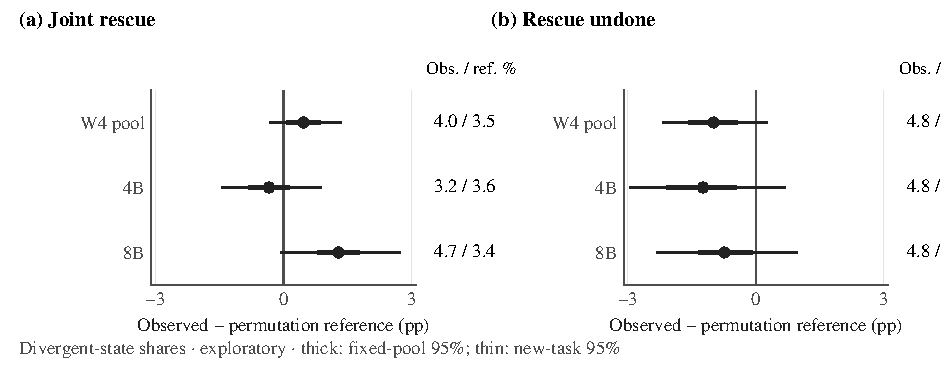
\includegraphics[width=\textwidth]{figures/f14_pattern_reference.pdf}
\caption{Joint rescue and rescue undone relative to label permutation on W4 divergent states. Thick lines show fixed-pool 95\% intervals; thin lines show new-task 95\% intervals. The right columns give observed and reference shares. These exploratory comparisons test enrichment, separately from the observed pattern counts in the main text. Values: Table~\ref{tab:patternref}.} % nocheck: interval conventions copied from the original caption; no outcome estimates here
\label{fig:modesfull}
\label{fig:modes}
\end{figure*}

\begin{table*}[t]
\centering% visual-layout-v1
\renewcommand{\arraystretch}{1.12}\fontsize{8.5}{10}\selectfont\setlength{\tabcolsep}{4pt}
% src: analysis/fork/out/dev_all_20261001T070326Z.md (two-sided table; W4:all pooled row); analysis/fork/out/dev_all_20261001T070326Z.json (pooled.W4:all:pooled_equal_weight.G.crossed_ci95)
\begin{tabular}{@{}lrrrrrll@{}}
\toprule
Cell & units & div. & $r$ & $d$ & $M$ & $\Gall$ [fixed pool] & [new tasks] \\
\midrule
q4 GPTQ-W4 & 85$\times$20 & 1102 & 6.8 & 8.7 & 15.5 & $-1.9$ [$-3.7$, $-0.1$] & [$-6.8$, $+2.7$] \\
q4 AWQ-style W4  & 85$\times$20 & 1439 & 9.8 & 10.1 & 19.9 & $-0.3$ [$-2.2$, $+1.6$] & [$-5.4$, $+5.2$] \\
q8 GPTQ-W4 & 85$\times$20 & 1473 & 10.4 & 7.5 & 17.9 & $+2.9$ [$+1.4$, $+4.4$] & [$-2.9$, $+9.2$] \\
q8 AWQ-style W4  & 85$\times$20 & 1562 & 11.4 & 9.5 & 20.9 & $+1.9$ [$-0.6$, $+4.3$] & [$-3.9$, $+8.1$] \\
W4 pool    & 85$\times$20 & & 9.6 & 9.0 & 18.6 & $+0.7$ [$-0.3$, $+1.6$] & [$-2.1$, $+3.4$] \\
\midrule
q4 KV8 & 85$\times$22 & 593 & 3.1 & 3.4 & 6.5 & $-0.3$ [$-1.7$, $+1.0$] & [$-3.0$, $+2.3$] \\
q8 KV8 & 85$\times$22 & 855 & 4.3 & 3.7 & 8.1 & $+0.6$ [$-0.4$, $+1.6$] & [$-1.9$, $+3.0$] \\
\midrule
q4 GPTQ-W3$^s$ & 85$\times$3 & 232 & 9.0 & 10.2 & 19.2 & $-1.2$ [$-7.0$, $+4.7$] & [$-8.6$, $+5.9$] \\
q4 KV4-rot$^s$ & 85$\times$3 & 233 & 11.8 & 7.1 & 18.8 & $+4.7$ [$-4.1$, $+13.5$] & [$-3.1$, $+12.9$] \\
q8 GPTQ-W3$^s$ & 85$\times$3 & 242 & 10.2 & 8.2 & 18.4 & $+2.0$ [$-12.5$, $+16.4$] & [$-6.3$, $+11.8$] \\
q8 KV4-rot$^s$ & 85$\times$3 & 239 & 11.8 & 8.6 & 20.4 & $+3.1$ [$-14.5$, $+20.8$] & [$-5.9$, $+12.9$] \\
q8 RTN-W3$^s$ & 85$\times$3 & 255 & 3.1 & 3.5 & 6.7 & $-0.4$ [$-3.8$, $+3.0$] & [$-4.7$, $+3.9$] \\
\bottomrule
\end{tabular}
\caption{Replacing Q's first tool-structure-divergent action while Q continues, \tautwo{} retail/airline panel (pp). Denominator: the full pool of tasks $\times$ complete blocks; units without a Bank P state count as zero. div.\ = Bank P states. $\Gall=r-d$ is a local replacement effect, \emph{not} the end-to-end success difference (Appendix~\ref{app:e2e}). Fixed pool: block bootstrap ($\ge$10 blocks) or $t$ over block means; new tasks: crossed task$\times$block bootstrap. $^s$stress cell, 3 blocks.}
\label{tab:r1}
\end{table*}

% GENERATED by tools/gen_ghf_combined.py; display only, no analysis changes.
% src: analysis/fork/out/ghf_20261001T211519Z.json; analysis/fork/out/ghf_20261001T211519Z.md; analysis/fork/out/ghf_multiplicity_20261001T225727Z.md
\begin{table*}[t]
\centering\fontsize{9}{11}\selectfont
\renewcommand{\arraystretch}{1.15}\setlength{\tabcolsep}{4pt} % nocheck: layout
\begin{tabular*}{\textwidth}{@{\extracolsep{\fill}}llllll@{}}
\toprule
Cell & states & $G$ (action) & $H$ (continuation) & $F$ (joint) & $G-H$ \\
\midrule
q4 GPTQ-W4 & 1102 & \shortstack[l]{$-2.9$ [$-5.7$, $-0.2$]\\{}[$-10.3$, $+4.2$]} & \shortstack[l]{$+0.7$ [$-1.6$, $+3.0$]\\{}[$-4.0$, $+6.0$]} & \shortstack[l]{$-2.5$ [$-5.3$, $+0.2$]\\{}[$-9.9$, $+4.7$]} & \shortstack[l]{$-3.6$ [$-6.6$, $-0.6$]\\{}[$-11.2$, $+3.6$]} \\
\addlinespace[1pt] % nocheck: layout
q4 AWQ-style W4 & 1439 & \shortstack[l]{$-0.3$ [$-2.6$, $+1.9$]\\{}[$-6.5$, $+6.1$]} & \shortstack[l]{$+0.9$ [$-1.1$, $+2.9$]\\{}[$-3.7$, $+5.5$]} & \shortstack[l]{$-0.8$ [$-3.3$, $+1.6$]\\{}[$-7.4$, $+5.8$]} & \shortstack[l]{$-1.3$ [$-3.0$, $+0.6$]\\{}[$-7.7$, $+5.1$]} \\
\addlinespace[1pt] % nocheck: layout
q8 GPTQ-W4 & 1473 & \shortstack[l]{$+3.3$ [$+1.6$, $+5.0$]\\{}[$-3.3$, $+10.5$]} & \shortstack[l]{$+0.4$ [$-1.2$, $+1.9$]\\{}[$-3.8$, $+4.9$]} & \shortstack[l]{$+5.4$ [$+3.5$, $+7.2$]\\{}[$-2.0$, $+13.0$]} & \shortstack[l]{$+2.9$ [$+1.3$, $+4.7$]\\{}[$-3.2$, $+9.3$]} \\
\addlinespace[1pt] % nocheck: layout
q8 AWQ-style W4 & 1562 & \shortstack[l]{$+2.1$ [$-0.6$, $+4.7$]\\{}[$-4.1$, $+8.7$]} & \shortstack[l]{$-1.3$ [$-3.5$, $+0.9$]\\{}[$-7.1$, $+4.6$]} & \shortstack[l]{$+0.6$ [$-1.5$, $+2.7$]\\{}[$-6.2$, $+7.3$]} & \shortstack[l]{$+3.4$ [$+1.5$, $+5.2$]\\{}[$-1.6$, $+8.6$]} \\
\addlinespace[1pt] % nocheck: layout
W4 pool & 5576 & \shortstack[l]{$+0.5$ [$-0.7$, $+1.7$]\\{}[$-2.9$, $+3.8$]} & \shortstack[l]{$+0.2$ [$-1.3$, $+1.6$]\\{}[$-2.7$, $+2.8$]} & \shortstack[l]{$+0.7$ [$-0.6$, $+2.1$]\\{}[$-3.1$, $+4.4$]} & \shortstack[l]{$+0.4$ [$-0.8$, $+1.7$]\\{}[$-3.1$, $+3.7$]} \\
\addlinespace[1pt] % nocheck: layout
\midrule
q4 KV8 & 593 & \shortstack[l]{$-1.0$ [$-5.3$, $+3.2$]\\{}[$-9.4$, $+7.3$]} & \shortstack[l]{$-2.5$ [$-4.5$, $-0.5$]\\{}[$-6.4$, $+1.1$]} & \shortstack[l]{$-1.2$ [$-4.7$, $+2.3$]\\{}[$-9.3$, $+7.7$]} & \shortstack[l]{$+1.5$ [$-3.1$, $+6.0$]\\{}[$-7.1$, $+9.7$]} \\
\addlinespace[1pt] % nocheck: layout
q8 KV8 & 855 & \shortstack[l]{$+1.3$ [$-0.9$, $+3.4$]\\{}[$-4.0$, $+6.9$]} & \shortstack[l]{$-0.4$ [$-2.1$, $+1.5$]\\{}[$-3.5$, $+2.9$]} & \shortstack[l]{$+2.5$ [$+0.0$, $+5.1$]\\{}[$-3.5$, $+8.1$]} & \shortstack[l]{$+1.6$ [$-0.6$, $+3.9$]\\{}[$-3.8$, $+7.2$]} \\
\addlinespace[1pt] % nocheck: layout
KV8 pool & 1448 & \shortstack[l]{$+0.1$ [$-2.8$, $+3.0$]\\{}[$-5.3$, $+5.6$]} & \shortstack[l]{$-1.4$ [$-2.7$, $-0.1$]\\{}[$-3.7$, $+0.9$]} & \shortstack[l]{$+0.6$ [$-1.8$, $+3.1$]\\{}[$-4.5$, $+5.8$]} & \shortstack[l]{$+1.6$ [$-1.2$, $+4.1$]\\{}[$-3.8$, $+6.6$]} \\
\addlinespace[1pt] % nocheck: layout
\midrule
q4 GPTQ-W3$^s$ & 232 & \shortstack[l]{$-1.3$ [$-7.7$, $+5.0$]\\{}[$-9.7$, $+6.6$]} & \shortstack[l]{$+4.3$ [$-10.7$, $+19.4$]\\{}[$-6.6$, $+14.5$]} & \shortstack[l]{$+1.3$ [$-1.9$, $+4.4$]\\{}[$-6.8$, $+9.4$]} & \shortstack[l]{$-5.6$ [$-15.0$, $+3.7$]\\{}[$-15.0$, $+4.0$]} \\
\addlinespace[1pt] % nocheck: layout
q4 KV4-rot$^s$ & 233 & \shortstack[l]{$+5.2$ [$-4.5$, $+14.9$]\\{}[$-3.4$, $+14.2$]} & \shortstack[l]{$+9.4$ [$+5.1$, $+13.7$]\\{}[$+2.1$, $+17.0$]} & \shortstack[l]{$+12.4$ [$+11.0$, $+13.9$]\\{}[$+3.0$, $+21.6$]} & \shortstack[l]{$-4.3$ [$-18.3$, $+9.8$]\\{}[$-13.5$, $+7.0$]} \\
\addlinespace[1pt] % nocheck: layout
q8 GPTQ-W3$^s$ & 242 & \shortstack[l]{$+2.1$ [$-13.3$, $+17.2$]\\{}[$-6.7$, $+12.1$]} & \shortstack[l]{$+0.4$ [$-7.4$, $+8.2$]\\{}[$-7.2$, $+8.1$]} & \shortstack[l]{$+2.1$ [$-7.4$, $+11.4$]\\{}[$-6.6$, $+11.8$]} & \shortstack[l]{$+1.7$ [$-9.1$, $+12.3$]\\{}[$-7.7$, $+11.2$]} \\
\addlinespace[1pt] % nocheck: layout
q8 KV4-rot$^s$ & 239 & \shortstack[l]{$+3.3$ [$-15.4$, $+21.9$]\\{}[$-6.6$, $+13.8$]} & \shortstack[l]{$-0.8$ [$-18.2$, $+16.3$]\\{}[$-11.2$, $+8.5$]} & \shortstack[l]{$+4.6$ [$-16.0$, $+25.0$]\\{}[$-6.6$, $+15.9$]} & \shortstack[l]{$+4.2$ [$+2.5$, $+5.8$]\\{}[$-3.3$, $+12.2$]} \\
\addlinespace[1pt] % nocheck: layout
q8 RTN-W3$^s$ & 255 & \shortstack[l]{$-0.4$ [$-3.8$, $+3.0$]\\{}[$-4.7$, $+3.9$]} & \shortstack[l]{$+15.3$ [$+0.7$, $+29.9$]\\{}[$+5.9$, $+25.9$]} & \shortstack[l]{$+18.4$ [$+16.7$, $+20.1$]\\{}[$+9.4$, $+28.2$]} & \shortstack[l]{$-15.7$ [$-27.5$, $-3.9$]\\{}[$-24.7$, $-7.1$]} \\
\addlinespace[1pt] % nocheck: layout
\bottomrule
\end{tabular*}
\caption{Upgrade gains on divergent states (pp). In each two-line cell, the first line gives the estimate and fixed-pool 95\% interval; the second gives the new-task crossed 95\% interval. $G$, $H$ and $F$ compare action-only, continuation-only and joint replacement with QQ. Fixed-pool intervals use a block bootstrap over 20--22 blocks, or a $t$ interval over three blocks for $^s$stress configurations. Pools average within-configuration estimates equally; stress configurations are separate.}
\label{tab:ghf}
\label{tab:ghf-crossed}
\end{table*}

% GENERATED by tools/gen_ghf_combined.py; display only, no analysis changes.
% src: analysis/fork/out/ghf_20261001T211519Z.json; analysis/fork/out/ghf_20261001T211519Z.md; analysis/fork/out/ghf_multiplicity_20261001T225727Z.md
\begin{table*}[t]
\centering\fontsize{9}{11}\selectfont
\renewcommand{\arraystretch}{1.15}\setlength{\tabcolsep}{4pt} % nocheck: layout
\begin{tabular*}{\textwidth}{@{\extracolsep{\fill}}llllll@{}}
\toprule
Cell & $F-G$ & $F-H$ & off-diag.\ \% & rev.\ \% & mean $I$ \\
\midrule
q4 GPTQ-W4 & \shortstack[l]{$+0.5$ [$-1.2$, $+2.2$]\\{}[$-4.7$, $+6.1$]} & \shortstack[l]{$-3.2$ [$-6.4$, $+0.2$]\\{}[$-11.1$, $+4.4$]} & 25.0 & 2.6 & $+0.3$ \\
\addlinespace[1pt] % nocheck: layout
q4 AWQ-style W4 & \shortstack[l]{$-0.4$ [$-2.4$, $+1.5$]\\{}[$-6.2$, $+5.4$]} & \shortstack[l]{$-1.7$ [$-3.6$, $+0.4$]\\{}[$-8.7$, $+4.7$]} & 29.3 & 3.1 & $+1.3$ \\
\addlinespace[1pt] % nocheck: layout
q8 GPTQ-W4 & \shortstack[l]{$+2.1$ [$+0.2$, $+4.0$]\\{}[$-3.0$, $+7.1$]} & \shortstack[l]{$+5.0$ [$+3.2$, $+6.8$]\\{}[$-2.0$, $+12.5$]} & 22.9 & 2.7 & $-1.7$ \\
\addlinespace[1pt] % nocheck: layout
q8 AWQ-style W4 & \shortstack[l]{$-1.5$ [$-4.2$, $+0.8$]\\{}[$-7.6$, $+4.2$]} & \shortstack[l]{$+1.9$ [$-0.1$, $+3.8$]\\{}[$-3.8$, $+7.5$]} & 30.5 & 4.2 & $+0.3$ \\
\addlinespace[1pt] % nocheck: layout
W4 pool & \shortstack[l]{$+0.2$ [$-1.0$, $+1.2$]\\{}[$-2.8$, $+3.1$]} & \shortstack[l]{$+0.5$ [$-1.0$, $+2.1$]\\{}[$-3.5$, $+4.5$]} & 26.9 & 3.2 & $+0.0$ \\
\addlinespace[1pt] % nocheck: layout
\midrule
q4 KV8 & \shortstack[l]{$-0.2$ [$-3.5$, $+3.7$]\\{}[$-5.7$, $+5.3$]} & \shortstack[l]{$+1.3$ [$-2.5$, $+4.9$]\\{}[$-6.7$, $+9.5$]} & 15.7 & 1.2 & $-2.4$ \\
\addlinespace[1pt] % nocheck: layout
q8 KV8 & \shortstack[l]{$+1.2$ [$-0.5$, $+3.2$]\\{}[$-2.5$, $+5.0$]} & \shortstack[l]{$+2.8$ [$+0.3$, $+5.5$]\\{}[$-3.1$, $+8.7$]} & 14.9 & 1.2 & $-1.5$ \\
\addlinespace[1pt] % nocheck: layout
KV8 pool & \shortstack[l]{$+0.5$ [$-1.6$, $+2.8$]\\{}[$-2.8$, $+3.9$]} & \shortstack[l]{$+2.1$ [$-0.2$, $+4.2$]\\{}[$-3.0$, $+7.3$]} & 15.3 & 1.2 & $-1.9$ \\
\addlinespace[1pt] % nocheck: layout
\midrule
q4 GPTQ-W3$^s$ & \shortstack[l]{$+2.6$ [$-0.6$, $+5.8$]\\{}[$-5.2$, $+10.5$]} & \shortstack[l]{$-3.0$ [$-15.1$, $+9.1$]\\{}[$-12.2$, $+6.6$]} & 31.5 & 3.9 & $+1.7$ \\
\addlinespace[1pt] % nocheck: layout
q4 KV4-rot$^s$ & \shortstack[l]{$+7.3$ [$-2.0$, $+16.5$]\\{}[$-1.3$, $+17.1$]} & \shortstack[l]{$+3.0$ [$-1.9$, $+8.0$]\\{}[$-6.2$, $+12.2$]} & 33.0 & 1.7 & $+2.1$ \\
\addlinespace[1pt] % nocheck: layout
q8 GPTQ-W3$^s$ & \shortstack[l]{$+0.0$ [$-11.0$, $+11.1$]\\{}[$-9.1$, $+9.1$]} & \shortstack[l]{$+1.7$ [$-0.1$, $+3.4$]\\{}[$-6.8$, $+11.0$]} & 23.1 & 4.5 & $+0.4$ \\
\addlinespace[1pt] % nocheck: layout
q8 KV4-rot$^s$ & \shortstack[l]{$+1.3$ [$-1.8$, $+4.3$]\\{}[$-7.2$, $+9.9$]} & \shortstack[l]{$+5.4$ [$+0.8$, $+10.0$]\\{}[$-2.5$, $+14.6$]} & 31.0 & 4.6 & $-2.1$ \\
\addlinespace[1pt] % nocheck: layout
q8 RTN-W3$^s$ & \shortstack[l]{$+18.8$ [$+13.8$, $+23.9$]\\{}[$+10.2$, $+27.8$]} & \shortstack[l]{$+3.1$ [$-13.0$, $+19.2$]\\{}[$-7.1$, $+13.3$]} & 29.0 & 0.4 & $-3.5$ \\
\addlinespace[1pt] % nocheck: layout
\bottomrule
\end{tabular*}
\caption{Paired mode contrasts and outcome patterns on the states of Table~\ref{tab:ghf}. Two-line cells give fixed-pool and new-task 95\% intervals in that order. Off-diag.: $\DQ\ne\DB$; rev.: $\DQ=-\DB\ne0$; interaction $I=\DQ-\DB$. Intervals are unadjusted. The four core W4 $G-H$ tests form a Holm family: q4 GPTQ-W4 has adjusted $p=.069$; all four new-task intervals cover zero. A positive $G-H$ compares two upgrades, not either upgrade against QQ.}
\label{tab:ghf-patterns}
\end{table*}



\label{app:r2main}

\subsection{The Two Illustrative Rescue Patterns} % nocheck: heading
\label{app:offdiag}

Everything in this section is exploratory and post hoc. It uses the four outcomes of each divergent state in the order BB, BQ, QB, QQ; $k$ is the number of successful arms.

\paragraph{Joint rescue and rescue undone against the reference.} A label-permutation reference for the two named patterns keeps $k$ for every state and permutes the four outcome labels uniformly: \texttt{1000} then has probability $1/4$ at $k=1$, and rescue undone (\texttt{0100} or \texttt{0110}) has $1/4$ at $k=1$ plus $1/6$ at $k=2$, so the reference shares are $P(k{=}1)/4$ and $P(k{=}1)/4+P(k{=}2)/6$, computed on the same states and bootstrap draws as the observed shares (Table~\ref{tab:patternref}). In the \tautwo{} W4 pool, joint rescue exceeds the reference by $+0.47$\pp{} on the fixed task pool ([$+0.06$, $+0.87$]), but the new-task interval spans zero ([$-0.33$, $+1.37$]); rescue undone is less frequent than the reference ($-0.99$ [$-1.58$, $-0.42]$; new tasks [$-2.19$, $+0.27$]). The excess of joint rescue is concentrated in the q8 cells, and no group shows a new-task excess of rescue undone. Because the reference keeps $k$ and does not model execution, a share near it says that the arrangement is about as common as a random arrangement of the same number of successes, not that the outcomes are noise or that the continuation is irrelevant. % src: analysis/fork/out/pattern_ref_20261005T134721Z.md (TL;DR; §1; §2; Method)
The observed shares in the W4 pool, with both intervals, are 4.0\% for joint rescue (fixed pool [3.5, 4.5]; new tasks [2.7, 5.3]) and 4.8\% for rescue undone ([4.1, 5.4]; [3.2, 6.5]). % src: analysis/fork/out/outcome_classes_20261004T143614Z.md (TL;DR; pool W4:all rows)

\begin{table*}[t]
\centering% visual-layout-v1
\renewcommand{\arraystretch}{1.12}\fontsize{8.5}{10}\selectfont\setlength{\tabcolsep}{4pt}
% src: analysis/fork/out/pattern_ref_20261005T134721Z.md (§1 fixed pool; §2 new tasks); analysis/fork/out/mistral_patterns_20261005T135040Z.md (§4, §5: A6:nonexact:pool)
\begin{tabular*}{\textwidth}{@{\extracolsep{\fill}}llllll@{}}
\toprule
\multicolumn{6}{@{}l}{\textbf{A. Joint rescue}} \\
\addlinespace[2pt]
Group & states & obs. & ref. & obs.$-$ref.\ [fixed pool] & [new tasks] \\
\midrule
\tautwo{} W4 pool & 5576 & 3.96 & 3.48 & $+0.47$ [$+0.06$, $+0.87$] & [$-0.33$, $+1.37$] \\
\quad q4 W4 cells & 2541 & 3.22 & 3.56 & $-0.34$ [$-0.83$, $+0.13$] & [$-1.46$, $+0.88$] \\
\quad q8 W4 cells & 3035 & 4.69 & 3.40 & $+1.29$ [$+0.79$, $+1.78$] & [$-0.07$, $+2.74$] \\
\tautwo{} KV8 pool & 1448 & 2.99 & 2.17 & $+0.81$ [$+0.10$, $+1.52$] & [$-0.51$, $+2.19$] \\
Telecom q8 W4 pool & 957 & 3.24 & 3.94 & $-0.70$ [$-1.46$, $+0.05$] & [$-2.47$, $+1.15$] \\
Same-precision W4 (Q$'$ as B) & 784 & 2.27 & 3.50 & $-1.23$ [$-2.47$, $-0.04$] & [$-2.88$, $+0.51$] \\
BF16, same blocks & 784 & 4.96 & 3.53 & $+1.43$ [$-0.40$, $+3.42$] & [$-0.90$, $+4.26$] \\
Mistral, own BF16 states$^m$ & 464 & 3.4 & 2.9 & $+0.5$ [$-2.4$, $+3.5$] & [$-2.0$, $+3.6$] \\
\bottomrule
\end{tabular*}
\par\vspace{6pt}
\begin{tabular*}{\textwidth}{@{\extracolsep{\fill}}llllll@{}}
\toprule
\multicolumn{6}{@{}l}{\textbf{B. Rescue undone}} \\
\addlinespace[2pt]
Group & states & obs. & ref. & obs.$-$ref.\ [fixed pool] & [new tasks] \\
\midrule
\tautwo{} W4 pool & 5576 & 4.80 & 5.78 & $-0.99$ [$-1.58$, $-0.42$] & [$-2.19$, $+0.27$] \\
\quad q4 W4 cells & 2541 & 4.77 & 6.01 & $-1.24$ [$-2.09$, $-0.45$] & [$-2.97$, $+0.69$] \\
\quad q8 W4 cells & 3035 & 4.82 & 5.56 & $-0.74$ [$-1.35$, $-0.07$] & [$-2.34$, $+0.98$] \\
\tautwo{} KV8 pool & 1448 & 2.31 & 4.58 & $-2.28$ [$-2.98$, $-1.58$] & [$-3.62$, $-0.98$] \\
Telecom q8 W4 pool & 957 & 4.18 & 5.13 & $-0.95$ [$-1.70$, $-0.20$] & [$-2.63$, $+0.61$] \\
Same-precision W4 (Q$'$ as B) & 784 & 5.77 & 5.75 & $+0.02$ [$-2.33$, $+2.25$] & [$-2.66$, $+2.92$] \\
BF16, same blocks & 784 & 3.82 & 6.14 & $-2.32$ [$-4.46$, $-0.19$] & [$-4.68$, $+0.17$] \\
Mistral, own BF16 states$^m$ & 464 & 4.0 & 4.7 & $-0.7$ [$-2.0$, $+0.7$] & [$-3.0$, $+1.9$] \\
\bottomrule
\end{tabular*}
\par\vspace{6pt}
\caption{Joint rescue and rescue undone against the conditional label-permutation reference (keeps the number $k$ of successful branches per state), \% of divergent states; exploratory, post hoc. 95\% intervals: fixed pool (block bootstrap for the 20- and 22-block \tautwo{} pools, $t$ over per-block ratios for fewer than 10 blocks: 6, or 5 for Mistral), new tasks (crossed task$\times$block). Same-precision rows each fork at their own first divergence. $^m$States whose actions differ, on BF16 trajectories (BB is the BF16 original), five blocks; not comparable with Bank P rows.}
\label{tab:patternref}
\end{table*}

\subsection{Task fragility}
\label{app:concentration}

All analyses in this subsection are exploratory and post hoc.

\paragraph{The consequences recur on the same tasks.} We split the 20 nonce blocks into two halves by an outcome-independent hash of the block name, ranked tasks by turnover on one half and measured the other half (Appendix Table~\ref{tab:fragility}). The 17 most fragile tasks (top 20\%) carry 41.0\% (crossed [26.6, 55.9]) and 42.3\% ([27.0, 57.5]) of the held-out turnover in the two directions, against 20\% if fragility did not persist. Their turnover is 38.7\%, while the other 68 tasks still turn over 13.7\%. Both groups have rescues and damages; neither group's net gain is resolved under the crossed interval. This replicates fragility on other nonces of the same tasks; it does not predict which new tasks are fragile. % src: analysis/fork/out/task_fragility_20261005T134836Z.md (Split-half fragility, both directions); analysis/fork/out/task_fragility_split_20261005T134815Z.json; derived: 68=85-17

\begin{table*}[t]
\centering% visual-layout-v1
\renewcommand{\arraystretch}{1.12}\fontsize{8.5}{10}\selectfont\setlength{\tabcolsep}{4pt}
% src: analysis/fork/out/task_fragility_20261005T134836Z.md (Split-half fragility: define A -> estimate B)
\begin{tabular}{@{}llllll@{}}
\toprule
Tasks & & $r$ & $d$ & $M$ & $\Gall$ \\
\midrule
fragile & est. & 21.1 & 17.6 & 38.7 & $+3.4$ \\
(top 20\%) & $t$ & [18.6, 23.5] & [14.3, 21.0] & [34.9, 42.6] & [$-1.0$, $+7.9$] \\
 & crossed & [14.8, 28.1] & [12.4, 23.3] & [32.3, 45.7] & [$-7.1$, $+13.7$] \\
\midrule
rest & est. & 6.5 & 7.2 & 13.7 & $-0.7$ \\
 & $t$ & [5.2, 7.8] & [6.2, 8.3] & [12.5, 14.9] & [$-2.7$, $+1.2$] \\
 & crossed & [4.4, 9.0] & [4.8, 9.9] & [10.2, 17.5] & [$-4.1$, $+2.4$] \\
\bottomrule
\end{tabular}
\caption{Repeatable task fragility (exploratory, post hoc; four \tautwo{} W4 cells, equal weight). Tasks are ranked by turnover on one hash-defined half of the 20 nonce blocks and measured on the other half (pp of units; 95\% intervals, $t$ over held-out blocks and crossed task$\times$block; direction A to B shown). A replication on other nonces of the same tasks, not a prediction for new tasks. Reverse direction: text.}
\label{tab:fragility}
\end{table*}

\paragraph{Split-half fragility (Table~\ref{tab:fragility}).} The halves are assigned by an outcome-independent hash of the block name (sha256 of a fixed prefix and the block name, mod 2), written to a file before this post hoc analysis loaded outcomes; fragility is a task's mean turnover over the four W4 cells and the defining half's blocks, and ties at the top-20\% threshold are broken by a hash. In the reverse direction (rank on the second half, estimate on the first), the 17 fragile tasks turn over 39.0\% ($t$ [34.2, 43.9]) and carry 42.3\% of the held-out turnover, the other tasks 13.3\%; the fragile tasks' net gain is $+3.7$\pp{} ($t$ [$+0.6$, $+6.9$]; crossed [$-5.0$, $+12.4$]) and the rest's $+0.5$. Ranking tasks by BF16 success instead (tertiles on one half) also separates turnover: the hardest tertile turns over 6.7--10.0\% and the others 25.4--27.3\%, with no net gain resolved under the crossed interval. % src: analysis/fork/out/task_fragility_20261005T134836Z.md (Split-half B -> A; BF16 difficulty tertiles; Method); analysis/fork/out/task_fragility_split_20261005T134815Z.json




\section{What Does Higher Precision Add?}
\label{app:sameprec}

Per model (final analysis set, $K=6$), the turnover difference is $\Delta M=+0.6$ [$-3.1$, $+4.3$]\pp{} in q4 and $-2.5$ [$-5.6$, $+0.5$] in q8 (fixed pool, 95\%), with crossed intervals [$-5.5$, $+6.9$] and [$-7.3$, $+2.7$]. Within $\pm$3\pp{}, equivalence is shown for no per-model $\Delta M$ or $\Delta\Gall$; the q8 off-diagonal difference ($+0.40$, 90\% [$-2.12$, $+2.92$]) is the only per-model contrast inside the margin. The protocol originally mapped ``interval includes 0 and $|\Delta M|\le3$\pp{}'' to ``similar''; after the interim result had been seen, an amendment replaced that reading by two one-sided tests, which are stricter, and changed no estimate. % src: analysis/fork/out/sameprec_20261004T070601Z.md (Paired differences; Amendment A1 table; analysis set K = 6); docs/insights/SAMEPREC_PROTOCOL.md (Amendment A1)
Acceptance: every state in both designs passed Q replay and every branch passed the prefix and environment checks; QQ no-op samples passed 265/265 (precision) and 242/242 (same precision), and no directory was quarantined. At the unit level, $\kappa$ is 0.43 in q4 and 0.61 in q8; at the task level, cross-design agreement at matched noise is 0.765 of within-design replication. % src: analysis/fork/out/sameprec_20261004T070601Z.md (Acceptance); analysis/fork/out/sameprec_overlap_20261002T143218Z.md (Agreement; Task-level, pooled cross/within)

W3 stress check (\S\ref{sec:sameprec}; $K=3$): every state passed Q replay, QQ no-op samples passed 31/31 and 39/39, and no directory was quarantined. All branches passed the prefix and environment checks except one of 774 in q8 same precision: a Q$'$Q$'$ branch that ended in an agent-side context overflow, for which the harness records no prefix comparison; its environment hash and first replayed prompt match the frozen state, and by the protocol it counts as a failure, not an exclusion. % src: analysis/fork/out/sameprec_w3_20261004T070607Z.md (Acceptance); analysis/fork/out/sameprec_prefix_check_20261003T030004Z.md


\paragraph{Equivalence tests (W4).} The difference in turnover is $\Delta M=M-M'=-0.98$\pp{} (90\% CI [$-3.26$, $+1.30]$). No precision-specific excess was detected, but equivalence within $\pm$3\pp{} is not shown either (two one-sided tests, $p=0.067$), and the same holds for the net gain ($\Delta\Gall=-1.57$ [$-5.17$, $+2.04$], $p=0.230$) and, descriptively, for the off-diagonal share ($-1.210$ [$-4.09$, $+1.67$], $p=0.133$, as the mean of per-block ratios, which the interval and test use; $-1.216$ as the ratio of block sums). % src: analysis/fork/out/sameprec_20261004T070601Z.md (Amendment A1 table, pool rows); analysis/fork/out/sameprec_20261004T070601Z.json (tost_a1.consistency.d_offdiag: -1.21 stored at 3-decimal rounding); derived: 1.210=1.21

\paragraph{Overlap details (W4).} The two action-replacement flip sets share 107 units, against 76 [69, 84] under a within-task block shuffle that preserves task-level flip propensity. % src: analysis/fork/out/sameprec_overlap_20261002T143218Z.md (Overlap table; Agreement)
When B also takes over the continuation, rescue sets under the continuation-only contrast agree with $\kappa=0.20$, and 70\% of continuation-dependent units are continuation-dependent under one substitution only. % src: analysis/fork/out/sameprec_split_20261002T145148Z.md (Figure-panel table; §1; §2; §3)

\paragraph{Full substitution (W4).} Under full substitution B flips more units than Q$'$ (193 vs.\ 149; $+4.3$ [$+0.4$, $+8.3$]\pp{}, one of several contrasts); the net difference comes only from substitution-specific units and is not resolved ($\Delta G=-1.6$ [$-6.2$, $+3.0$]\pp{}). Only value measures on the same units reveal this structure. % src: analysis/fork/out/sameprec_split_20261002T145148Z.md (§3 net decomposition; cross-direction counts)

\paragraph{W3 stress pair.} The protocol's complete W3 panel (Q GPTQ-W3, Q$'$ a second W3 calibration draw; q4 and q8, $K=3$ blocks q3--q5, 510 units) is reported next to W4, never pooled with it. The same-precision substitution produces 17.3\pp{} of turnover, the BF16 substitution 18.8\pp{}; off-diagonal shares are 27.6\% and 27.3\%. % src: analysis/fork/out/sameprec_w3_20261004T070607Z.md (TL;DR; Full pool, pool rows); analysis/fork/out/sameprec_w3_split_20261003T024007Z.md (510 units); docs/insights/SAMEPREC_W3_PROTOCOL_20261002.md (K = 3, q3-q5)
$\Delta M=+1.6$\pp{} (95\% [$-0.66$, $+3.80$]) is unresolved: the preregistered $\pm$3\pp{} equivalence test fails ($p=0.055$); that the 90\% interval lies just above zero does not change this. $\Delta\Gall$ is equivalent within $\pm$3\pp{} only in the preregistered pooled population ($+1.2$, $p=0.017$); per model it is $+3.1$ (q4) and $-0.8$\pp{} (q8). The off-diagonal difference is $-0.288$ (ratio of block sums) or $-0.307$ (mean of per-block ratios, used by the interval and test: 90\% [$-11.0$, $+10.4]$, $p=0.27$). % src: analysis/fork/out/sameprec_w3_20261004T070607Z.md (Amendment A1 table; Paired differences); analysis/fork/out/sameprec_w3_20261004T070607Z.json (pooled.paired.dM.ci95; tost_a1.consistency.d_offdiag)
On the action side ($G$), rescued and harmed task$\times$block units overlap ($\kappa=0.60$, $0.68$); the designs may first diverge at different decisions, so this is unit overlap, not a same-state replication. Of 122 units whose $G$ outcome flips, 62 flip under both substitutions, 34 only under BF16 and 26 only under the other W3 checkpoint: 49\% respond to only one. Flip volume, affected units and net upgrade value must be measured separately. % src: analysis/fork/out/sameprec_w3_split_20261003T024007Z.md (Figure-panel table, G rows; TL;DR); derived: 122=62+34+26

\subsection{Common states: extra value of the BF16 action}
\paragraph{Common-state comparison: details.} Above, each design selects its own divergent states. A pre-registered comparison removes that difference: on 510 ordinary q8 states (85 tasks $\times$ 6 blocks, sampled by a fixed rule), the current action comes from B, from Q (GPTQ-W4, first checkpoint) or from Q$'$ (second checkpoint), and B or Q continues. $K(c)=V(\mathrm{B},c)-V(\mathrm{Q}',c)$ asks what B's action adds beyond another W4 action. A frozen rule claims value only if both intervals exclude zero (Holm), equivalence only if both lie within $\pm$3\pp{} (two one-sided tests). % src: docs/insights/COMMONSTATE_SOURCES_PROTOCOL.md (§2 design, §5 estimands, §6 frozen reading; A1.1); analysis/fork/out/commonstate_q8ext_20261003T231159Z.md (header); derived: 510=85*6
The design first ran three blocks, and that first look was unresolved (under Q's continuation $K=-0.4$\pp{}, 95\%: $t$ [$-9.3$, $+8.5$], bootstrap [$-3.5$, $+2.7$]; under B's $+2.4$\pp{}, [$-3.5$, $+8.2$], [$-0.8$, $+5.5$]). Three more blocks were then added. That decision followed the unresolved first look, so a dated amendment fixed the extension before any new outcome existed, and a two-look reading (Pocock levels from a normal approximation: about 97\% intervals for a difference and 94\% for equivalence), was designated confirmatory in that amendment. The Pocock constant is not calibrated for small-$k$ $t$ intervals, the task bootstrap or the joint rule, so the two-look reading carries no exact error guarantee; we therefore report it as a sensitivity analysis next to the ordinary intervals and claim neither an advantage nor equivalence unless both agree. % src: analysis/fork/out/commonstate_20261002T201612Z.md (Key estimand table); docs/insights/COMMONSTATE_SOURCES_PROTOCOL.md (A1 'What was known', A1.3, D2.2)
After the fixed extension (six blocks), B's action is not shown to be worth more than Q$'$'s, and equivalence is not established. Under Q's continuation, $K=+1.0$\pp{} (95\%: $t$ [$-3.5$, $+5.4$], bootstrap [$-1.2$, $+3.1$]; two-look 97\%: [$-4.2$, $+6.2$], [$-1.4$, $+3.5$]). Under B's, $K=+0.8$\pp{} (95\%: [$-1.8$, $+3.3$] for both; two-look 97\%: [$-2.2$, $+3.8$], [$-2.0$, $+3.7$]). For equivalence under B's continuation, the ordinary 90\% intervals lie within $\pm$3\pp{} ($t$ [$-1.2$, $+2.8$], bootstrap [$-1.4$, $+2.9$]) and the two-look 94\% intervals of the sensitivity analysis do not ($t$ [$-1.6$, $+3.2$]); because the extension followed the first look, we do not claim equivalence. Without the 26 states at which earlier studies had already produced outcomes, $K$ is $+0.5$ and $+0.8$\pp{}, also not resolved. % src: analysis/fork/out/commonstate_q8ext_20261003T231159Z.md (Key estimand table; Two-look reading table; Sensitivity without the D2.1 states); docs/insights/COMMONSTATE_SOURCES_PROTOCOL.md (D2.1)
Under Q's continuation, B's action flips $M=7.1$\% of outcomes (rescue 4.1, damage 2.9) for a net $\Delta=+1.2$\pp{} (95\%: $t$ [$-1.3$, $+3.6$]); Q$'$'s flips 8.0\% (4.1, 3.9) for $+0.2$\pp{} ([$-2.3$, $+2.7$]; within $\pm$3\pp{} by two one-sided tests). A second W4 checkpoint's action departs from Q's at least as often as B's does (agreement with Q's action 53.9\% against 55.7\%; B with Q$'$ 57.3\%; Figure~\ref{fig:commonstate}d). The interaction of $K$ with the continuation is $-0.2$\pp{} (95\%: $t$ [$-4.5$, $+4.1$], bootstrap [$-2.7$, $+2.4$]; secondary, not resolved). % src: analysis/fork/out/commonstate_q8ext_20261003T231159Z.md (Contrasts table, c = d1 rows; Action agreement; Interaction table, bf16 − d2 row)
\emph{q4, a separate prospective analysis.} The same design on Qwen3-4B planned three blocks. The frozen quarantine rule removed f01 (below), leaving 170 states. $K=-1.2$\pp{} under Q's continuation (bootstrap 95\% [$-5.9$, $+3.5$]) and $-2.4$\pp{} under B's ([$-6.5$, $+1.2$]), both not resolved. With two blocks the $t$ interval has one degree of freedom. Under Q's continuation the two block means happen to coincide, so it collapses to a point. That is a coincidence of two values, not a precise measurement or zero variance, and the reading rests on the bootstrap. % src: analysis/fork/out/commonstate_q4_20261004T001159Z.md (TL;DR; Key estimand table)
\emph{Identity checks.} Across both models, 1{,}238 of 1{,}240 reference and implicit identity checks passed. Both failures are one q4 state. There the substituted action was semantically identical to the original after parsing, but its token sequence differed in the order of keys inside a tool-call argument. The canonical comparison treats such actions as equal, but the chat template renders the order, so the next prompt differed and the continuation could not be a replay. Every check with a token-identical action passed (869/869). As the frozen rule requires, the block was removed. % src: analysis/fork/commonstate_replay_check/Q4_F01_IDENTITY.md (TL;DR; acceptance table); docs/insights/COMMONSTATE_ERRATA.md (E-2)
Changing outcomes is thus not improving them; this does not make precision irrelevant or the two actions equivalent.

\section{Trigger, Oracle and KL Detail (supports \texorpdfstring{\S\ref{sec:r4}}{the trigger result})}
\label{app:r3}

This appendix supports \S\ref{sec:r4}: the frozen Q-only trigger enriches outcome-changing decisions but does not select net-beneficial upgrades, and token KL tracks how often actions differ, not net value (exploratory, post hoc).

\subsection{The frozen trigger and its headroom}
\label{app:token}
Following \citet{lotfi2026quantized}, we scored every Bank U f01 state at the token level (1140 cell $\times$ state rows, 58 flips), teacher-forcing both models on the generated ids of $a_{\mathrm{B}}$ and $a_{\mathrm{Q}}$. We record truncated top-20 entropy, the top-1 margin and a top-20-union KL, not full entropy or KL. All analyses are exploratory, and f01 is development data. % src: analysis/fork/out/token_mech_20261001T185031Z.md (§0); docs/RESEARCH_LOG.md W88

\paragraph{Uncertainty is associated with divergence.} Q's entropy at the start of its action separates states where B and Q act differently from states where they act identically, with AUC 0.66--0.91 per sub-bank and model. Over all ordinary states, flips also sit at lower Q margins (U1: AUC 0.31 [0.22, 0.40] for q4, 0.24 [0.13, 0.36] for q8; stratified). % src: analysis/fork/out/token_mech_20261001T185031Z.md (§1a, §1b "differing vs exact"); docs/RESEARCH_LOG.md W88
Among already divergent U1 states, no Q-visible statistic has an interval excluding AUC 0.5; small-subset associations vary across state sources. This development diagnosis motivated the frozen margin rule, whose validation reuses the tasks with fresh nonce blocks. % src: analysis/fork/out/token_mech_20261001T185031Z.md (§1a differing_only); analysis/fork/out/token_mech_20261002T003130Z.md (§3)
On the secondary validation population, ordinary states from BF16 trajectories (U2B; f02/f03, 1020 rows, 75 outcome-changing states), the frozen rule captures 4, 11 and 35 outcome-changing states against 3.81, 8.35 and 16.07 expected at random ($p=.5404$ and $.1995$ at 5 and 10\%; the 20\% excess is resolved), with net gains of $-2$, $-1$ and $+5$ against random $+0.07$, $+1.10$ and $+2.48$. % src: analysis/fork/out/token_mech_20261002T003130Z.md (§3 Validation, U2B S_mm secondary)

\subsection{Matched references for the frozen trigger}
\label{app:oracle}

Table~\ref{tab:oracle} compares the frozen trigger of \S\ref{sec:r4} (frozen rule, unchanged) with two references on the same 1020 f02/f03 U1 rows, which hold 38 rescues and 31 damages. The \emph{matched action-replacement oracle} selects, per cell, exactly as many rows as the frozen rule did, taking only rows with $G>0$ and filling with $G=0$ rows when a cell has too few rescues; it never selects a damage. It is hindsight selection, not a policy. At the 10\% and 20\% budgets every rescue fits. % src: analysis/fork/out/oracle_trigger_20261002T024423Z.md (§1a)
The \emph{three-option menu oracle} $E[\max(G,H,F,0)]$ is the share of states where some arm beats QQ. On Bank P divergent states it is 0.202 over the four W4 cells (state-weighted, the one exception to the paper's equal-weight pools) against 0.117 for the action alone (1127 vs.\ 654 of 5576 states), and 0.191 vs.\ 0.113 over the six core cells. It is hindsight selection that also allows different replacement types, with different costs, so it is not a same-cost deployment comparison and not comparable with the action rule. % src: analysis/fork/out/oracle_trigger_20261002T024423Z.md (§1b)

The \emph{KL reference row} is a post-hoc auxiliary baseline. Its score is a truncated KL$(\mathrm{B}\|\mathrm{Q})$ over the union of both models' top-20 next-token sets plus a tail bucket, per $a_{\mathrm{Q}}$ token, teacher-forced on identical prompt ids. It needs a BF16 prefill of the prompt and $a_{\mathrm{Q}}$ at every decision (here 6709.3 prompt and 82.3 action tokens on average), so it is not Q-only. It captures turnover above chance (33 vs.\ 16.7 at 20\%) but no significant net gain (Holm $p=1.0$). Three aggregations over the $a_{\mathrm{Q}}$ tokens were fit on f01 only, with per-cell thresholds and the frozen rule's selection criterion; the maximum was chosen, and all of f02/f03 is reported. Because the f02/f03 outcomes had been seen, the row is post hoc, and it is not a DMR reproduction, which trains a router. % src: analysis/fork/out/oracle_trigger_20261002T024423Z.md (§2)


\begin{table*}[t]
\centering\scriptsize\setlength{\tabcolsep}{3pt}
% src: analysis/fork/out/oracle_trigger_20261002T024423Z.md (§1a action oracle; §2 validation table)
\begin{tabular}{@{}rrlllllll@{}}
\toprule
& & \multicolumn{3}{c}{same per-cell selection counts} & \multicolumn{4}{c}{KL reference (max.\ per-token KL; needs BF16; post hoc)} \\
Budget & sel. & oracle r/d/net (pp) & frozen r/d/net (pp) & net ratio & sel. & net vs.\ random ($p$; Holm) & r/d & turnover vs.\ random ($p$) \\
\midrule
5\%  & 50  & 34/0/$+34$ ($+3.33$) & 6/2/$+4$ ($+0.39$)   & 4/34 & 72  & $-1$ vs.\ $+0.45$ (.8337; 1.0000) & 5/6   & 11 vs.\ 4.58 (.0038) \\
10\% & 114 & 38/0/$+38$ ($+3.73$) & 7/5/$+2$ ($+0.20$)   & 2/38 & 126 & $+1$ vs.\ $+0.82$ (.5483; 1.0000) & 8/7   & 15 vs.\ 7.54 (.0048) \\
20\% & 222 & 38/0/$+38$ ($+3.73$) & 16/11/$+5$ ($+0.49$) & 5/38 & 257 & $+3$ vs.\ $+1.59$ (.3984; 1.0000) & 18/15 & 33 vs.\ 16.73 ($<10^{-4}$) \\
\bottomrule
\end{tabular}
\caption{Frozen Q-only trigger against a matched action-replacement oracle (hindsight; same per-cell selection counts) and a post-hoc KL reference row, on f02/f03 U1 (1020 rows). Net ratio: frozen net over oracle net (not a share of rescues; the frozen rule selects 6, 7 and 16 of the oracle's rescues). Random: matched-count per-cell random-trigger expectation; $p$: exact one-sided hypergeometric, Holm over the three budgets.}
\label{tab:oracle}
\end{table*}

\subsection{Fidelity, sensitivity and signed value}
\label{app:kl}

\paragraph{KL tracks action divergence and turnover, not net value.} On ordinary BF16-sourced states shared by every method (U2B), we compare methods by $D_{cc}=\YY{QB}-\YY{BB}$, Q's action against B's under the shared BF16 continuation, with turnover $M_{cc}$ (Appendix~\ref{app:panels}). These comparisons evaluate complete quantization configurations, including their calibration pipelines, rather than isolated algorithmic components. Across the eleven q8 configurations (descriptive Spearman), mean teacher-forced approximate token KL$(\mathrm{B}\|\mathrm{Q})$ is strongly associated with the action-difference rate ($\rho=0.99$) and with turnover ($\rho=0.925$ with $M_{cc}$). Conditional on the actions differing, its association with consequences is weak: $\rho=0.46$ with the flip rate given a difference, and within configurations a mean AUC of 0.46 for flips among differing actions, against 0.93 for separating differing from identical actions. It gives no reliable prediction of net value ($\rho=-0.44$ with $D_{cc}$), consistent with KL measuring the size of a disagreement rather than its direction \citep{nikolic2026displacement}. SpinQuant-W4A4 has lower KL than QuaRot-W4A4 (0.165 against 0.199), yet their pre-registered task-value contrast is unresolved ($+1.2$\pp{}, crossed [$-4.7$, $+7.1$]; Appendix~\ref{app:panels}). % src: analysis/fork/out/kl_decomp_20261005T000559Z.md (TL;DR; §2; §3); analysis/fork/out/newmethod_q8_20261004T051538Z.md; analysis/fork/out/newmethod_q8_20261004T051538Z.json (tau2.contrasts; fidelity.cells.*.KLu_mean); docs/insights/NEWMETHOD_PANEL_PROTOCOL.md (§2.1, §4, A1.2, A7); analysis/fork/out/backfill_20261003T193042Z.md (TL;DR 2; §2)

The following decomposition was added after panel results were read and is exploratory. On each cell's admitted states, exact action equality and deterministic continuation give
\[
M_{cc}=P(a_{\mathrm{Q}}\ne a_{\mathrm{B}})\,
P(\YY{QB}\ne\YY{BB}\mid a_{\mathrm{Q}}\ne a_{\mathrm{B}}).
\]
B's rescues $r_{cc}=P(\YY{BB}=1,\YY{QB}=0)$ and damages $d_{cc}=P(\YY{BB}=0,\YY{QB}=1)$ give $D_{cc}=d_{cc}-r_{cc}$. The decomposition separates how often an action changes from what a changed action does; it is diagnostic rather than a mechanism. % src: analysis/fork/out/kl_decomp_20261005T000559Z.md (§1); analysis/fork/kl_decomp.py

\paragraph{Approximate KL.} Both models are teacher-forced on identical prompt ids and B's action tokens. At each token, KL$(\mathrm{B}\|\mathrm{Q})$ uses the union of both top-20 sets and the forced token, plus one tail bucket per model. An in-union token missing from a model's top-20 receives min(the 20th probability, tail mass divided by the number of missing tokens). The state score averages over B's action tokens. This coarse distribution is not the full token distribution. % src: analysis/fork/out/kl_decomp_20261005T000559Z.md (§1); analysis/fork/kl_decomp.py

\paragraph{Across and within configurations.} Across eleven q8 cells, KL's descriptive Spearman correlation is 0.99 with the action-difference rate, 0.925 with $M_{cc}$, 0.81 with rescues and 0.93 with damages. It is 0.46 with the flip rate conditional on a difference and $-0.44$ with $D_{cc}$. Removing the three unquantized path controls (eight configurations) gives 0.98, 0.64 and $-0.52$ for the action-difference rate, conditional flip rate and $D_{cc}$. These configurations are not exchangeable draws. Within cells, the mean AUC is 0.93 for an action difference, 0.46 for a flip conditional on a difference and 0.55 for a rescue conditional on a flip; the last uses 3--39 flips per cell. These diagnostics establish no reliable predictor of net upgrade value. % src: analysis/fork/out/kl_decomp_20261005T000559Z.md (§2, §3)

\begin{table}[t]
\centering\scriptsize\setlength{\tabcolsep}{3pt}
% src: analysis/fork/out/kl_decomp_20261005T000559Z.md (§1 paired SpinQuant minus QuaRot W4A4); docs/insights/NEWMETHOD_PANEL_PROTOCOL.md
\begin{tabular}{@{}lll@{}}
\toprule
SpinQuant $-$ QuaRot & difference [fixed pool] & [new tasks] \\
\midrule
KL ($\times10^{-3}$) & $-34$ [$-57$, $-11$] & [$-56$, $-11$] \\
Action difference (pp) & $+0.8$ [$-11.4$, $+13.0$] & [$-8.2$, $+9.4$] \\
Flip given difference (pp) & $+2.7$ [$-10.2$, $+15.3$] & [$-7.5$, $+11.4$] \\
$D_{cc}$ (pp) & $+1.2$ [$-3.9$, $+6.2$] & [$-4.7$, $+7.1$] \\
\bottomrule
\end{tabular}
\caption{Paired diagnostic on 255 identical W4A4 states; 95\% intervals, $t$ over three block differences and crossed task$\times$block bootstrap. The KL reduction is resolved; the differences in the task quantities remain unresolved. The $D_{cc}$ row is primary contrast P2.}
\label{tab:fidelity-components}
\end{table}

\section{Where Do the Consequences Persist?}
\subsection{Ordinary states and the user simulator}
\label{app:ordinary}

\paragraph{Ordinary states turn over less, mostly through text under our simulator.} At ordinary states, replacing Q's action changes the outcome less often than at first tool-structure divergences (a descriptive comparison of different state populations, with no interval on the difference). Over blocks f01--f03 (task-equal; $t$ intervals over block means), $M$ per sub-bank is 7.8--9.0\% for the q4 W4 cells in U1 and U2B, 4.7--9.0\% for the q8 W4 cells and at most 4.7\% for KV8. The net gain lies within $\pm$2.8\pp{} (U1, U2B) and $\pm$5.0\pp{} (U2Q), and every interval covers zero (Appendix~\ref{app:banku}). % src: analysis/fork/out/bank_u_f01_f02_f03_20261002T003037Z.md (§2)
Identical actions never change the outcome, as determinism implies. Reused arms rest on canonical equality. All 4{,}114 such reuses were rendered with each model's chat template; 4{,}113 are token-identical. The remaining pair differs only in JSON key order, and its two cross arms, measured separately, gave the reused outcomes. % src: analysis/fork/reuse_audit/REUSE_AUDIT.md (TL;DR); analysis/fork/reuse_audit/REUSE_FIX_RESULT.md (TL;DR)
After deduplication, 150 of the 208 outcome-changing cell$\times$state rows ($\approx$72.1\%) are class (ii), the same tool structure with different text; 26 involve a different tool name, call count or argument (Table~\ref{tab:taxonomy}). % src: analysis/fork/out/bank_u_f01_f02_f03_20261002T003037Z.md (§3); derived: 150=45+28+44+25+10+6-5-3; 208=99+99+18-5-3; 72.1=100*(45+28+44+25+10+6-5-3)/(99+99+18-5-3); 26=1+11+4+9+0+1
The rows are not independent states: the three blocks repeat the same tasks, and each U2B/U2Q state appears once per cell of a model.
This is a \emph{composition share}: per instance, text, tool/argument and act/talk differences flip the outcome in 14.4\%, 18.2\% and 18.9\% of rows. Text dominates because it is common (1045 of 1357 differing rows), not because each text difference matters more. % src: analysis/fork/out/bank_u_f01_f02_f03_20261002T003037Z.md (§3); derived: 14.4=100*(45+28+44+25+10+6-5-3)/(309+202+277+199+63+33-24-14); 1045=309+202+277+199+63+33-24-14; 18.2=100*(1+11+4+9+0+1)/(19+47+24+40+5+11-1-2); 18.9=100*(10+4+3+14+1+0)/(38+33+34+56+4+7-1-2); 1357=309+202+277+199+63+33-24-14+19+47+24+40+5+11-1-2+38+33+34+56+4+7-1-2

\paragraph{Sensitivity to the user simulator.} Text actions act through the user simulator, and changing the simulator moves $\tau$-bench outcomes by 9--15 points \citep{seshadri2026lost,jain2026userproxybench}. % src: outputs/.drafts/storyline-v7-lit.md (rows 23-24)
We froze a control before running it: the 39 deduplicated class-(ii) flips of block f01 and 39 matched non-flip states. Their BQ and QQ branches were each re-run three times with a different user simulator, Sonnet 5.5, answering through a file relay from Claude Code subagents (reproducibility limits in the Limitations). % src: docs/RESEARCH_LOG.md W90, W91 (manifests/fork/simctrl_v3.json)
Judged by the sign of the replicate mean, only 7 of the 39 flips keep their direction (95\% CI 0.075--0.335). Six reverse, and 26 vanish (15 both succeed, 2 both fail, 9 ties). Among the matched non-flip states, 11 of 39 become flips (0.15--0.45). Replicates of the same arm disagree in 41\% of flip arms and in 21--26\% of control arms. % src: analysis/fork/out/simctrl_20261001T212742Z.md
\textbf{The Bank U text-difference outcome labels did not reproduce reliably under this alternative relay setting.} The control changes three things at once (simulator model, sampling, relay interface), so it cannot say which of them changed the labels.

\paragraph{Sensitivity of the four-branch results.}
\label{app:simctrlpmain}
Before running, we sampled 80 Bank P states without outcome information (20 per W4 cell, stratified by domain and block) and re-ran all four arms five times each with Sonnet 5.5 as the user, one isolated single-request call per user turn (7896 calls; all integrity checks passed). % src: analysis/fork/out/simctrl_p_20261002T015200Z.md; manifests/fork/simctrl_p_v1.json
Per-state arm outcomes track the original single runs (correlation 0.63--0.68). Pooled over cells, $G=-3.0$ [$-10.2$, $+4.8$], $H=+5.5$ [$+0.0$, $+11.2$] and $G-H=-8.5$ [$-14.8$, $-2.8$]\pp{} under Sonnet, against $G-H=-2.5$ [$-11.2$, $+6.2$] on the same states under the original simulator (change $-6.0$ [$-16.2$, $+4.2$]). % src: analysis/fork/out/simctrl_p_20261002T015200Z.md (pool, all batches)
With 20 states per cell, this control cannot resolve the few-pp contrasts of Table~\ref{tab:ghf} (on this sample even the original simulator gives $G-H=0.0$ in both q8 W4 cells), so it neither confirms nor reverses the within-cell orderings. % src: analysis/fork/out/simctrl_p_20261002T015200Z.md (q8 cells)


\paragraph{Bank P and Bank U measure different quantities.} Bank P skips text-only differences by design, yet these make up 150 of the 208 outcome-changing rows at ordinary states, and their labels did not reproduce under a second simulator (Appendix~\ref{app:banku}; \S\ref{sec:scope}). Including text actions requires a simulator control before their consequences are reported as a property of the action. % src: analysis/fork/out/bank_u_f01_f02_f03_20261002T003037Z.md (§3); analysis/fork/out/simctrl_20261001T212742Z.md; derived: 150=45+28+44+25+10+6-5-3; 208=99+99+18-5-3


\subsection{Bank U per Sub-Bank}
\label{app:banku}

Table~\ref{tab:banku} gives the per-state turnover behind Appendix~\ref{app:ordinary}, over blocks f01--f03. Exact action agreement is 0.43--0.83 per cell and sub-bank. % src: analysis/fork/out/bank_u_f01_f02_f03_20261002T003037Z.md (column "exact")

\begin{table}[h]
\centering\scriptsize\setlength{\tabcolsep}{3.5pt}
% src: analysis/fork/out/bank_u_f01_f02_f03_20261002T003037Z.md (§2 Native estimates, task-equal; r and d counts)
\begin{tabular}{@{}lccc@{}}
\toprule
Cell & U1 ($n{=}255$) & U2B ($n{=}255$) & U2Q ($n{=}60$) \\
\midrule
q4 GPTQ-W4 & .090 (11/12) & .082 (10/11) & .083 (4/1)$^\ast$ \\
q4 AWQ-W4  & .082 (7/14) & .078 (7/13) & .083 (3/2) \\
q4 KV8     & .047 (4/8) & .039 (5/5) & .017 (0/1) \\
q8 GPTQ-W4 & .047 (8/4) & .067 (9/8) & .050 (3/0)$^\ast$ \\
q8 AWQ-W4  & .086 (14/8) & .090 (15/8) & .067 (3/1) \\
q8 KV8     & .035 (5/4) & .031 (6/2) & 0 (0/0) \\
\bottomrule
\end{tabular}
\caption{Bank U, blocks f01--f03: per-state turnover $M$ (rescues/damages), task-equal (one state per task and block; 85/85/20 states per block). $G$ lies within $\pm0.028$ in U1 and U2B and within $\pm0.050$ in U2Q, and every interval includes 0. Intervals are $t$ intervals over the three block means and are wide (e.g.\ q4 GPTQ-W4 U1: .090 [.029, .151]). $^\ast$GPTQ-W4's U2Q states are its own U1 states, with concordant outcomes on 20/20 duplicates per block; they are counted once in cross-sub-bank totals.}
\label{tab:banku}
\end{table}

\begin{table}[h]
\centering\scriptsize\setlength{\tabcolsep}{2.6pt}
% src: analysis/fork/out/bank_u_f01_f02_f03_20261002T003037Z.md (§3 class composition and consequence per sub-bank; per cell; comparator block, unique states)
\begin{tabular}{@{}lllll@{}}
\toprule
& (i) identical & (ii) same tool & (iii) different & (iv) act vs.\ \\
Model:sub & & structure, text & tool or args & talk \\
\midrule
q4:U1  & 399: 0 & 309: 45 (.146) & 19: 1 (.053) & 38: 10 (.263) \\
q8:U1  & 483: 0 & 202: 28 (.139) & 47: 11 (.234) & 33: 4 (.121) \\
q4:U2B & 430: 0 & 277: 44 (.159) & 24: 4 (.167) & 34: 3 (.088) \\
q8:U2B & 470: 0 & 199: 25 (.126) & 40: 9 (.225) & 56: 14 (.250) \\
q4:U2Q & 108: 0 & 63: 10 (.159)$^\ast$ & 5: 0 & 4: 1 (.250) \\
q8:U2Q & 129: 0 & 33: 6 (.182)$^\ast$ & 11: 1 (.091) & 7: 0 \\
\midrule
unique rows & 1943: 0 & 1045: 150 (.144) & 143: 26 (.182) & 169: 32 (.189) \\ % derived: 1045=309+202+277+199+63+33-24-14; 150=45+28+44+25+10+6-5-3; 143=19+47+24+40+5+11-1-2; 26=1+11+4+9+0+1; 169=38+33+34+56+4+7-1-2; 32=10+4+3+14+1+0; .144=150/1045; .182=26/143; .189=32/169
\bottomrule
\end{tabular}
\caption{Which kind of action difference changes the outcome at ordinary states (Bank U, blocks f01--f03). Entries: ``state rows: outcome-changing rows (flip rate)'', pooled over the three cells of a model within a sub-bank. The last row counts each (cell, state) once: q4/q8 GPTQ-W4's U2Q states repeat their U1 states ($^\ast$ includes 5 and 3 repeated class-(ii) flips), so 216 flipping rows become 208. In block f01 alone the corresponding counts were 39 of 56 flips in class (ii), with rates .126/.109/.200 for (ii)/(iii)/(iv); the 58 f01 flips scored in Appendix~\ref{app:token} include the two duplicated U2Q rows. % src: analysis/fork/out/token_mech_20261001T185031Z.md (flips: 58); analysis/fork/out/bank_u_f01_f02_f03_20261002T003037Z.md (§3); analysis/fork/out/bank_u_f01_20261001T134456Z.md; docs/REPORT_GPT61_20261001_0915.md (correction 1: 39/56 after deduplication); derived: 216=99+99+18; 208=99+99+18-5-3
}
\label{tab:taxonomy}
\end{table}

\subsection{Models compared on their own ordinary states}
\label{app:mistral}
\paragraph{Mistral population, scoring and coverage.} The Mistral panel applies the same row rule to Mistral's own BF16 trajectories on the 85 retail and airline tasks. Seven BF16 source rows are missing because the source episode ended in an invalid tool call produced by the model itself (airline task 44 in all six blocks, airline task 13 in f01). A dated amendment, fixed from the BF16 source runs before any Mistral fork output existed, excludes both tasks in every block and cell, leaving 83 tasks. The selection was outcome-blind, but BF16 Mistral fails these tasks structurally, so the estimates describe this conditional population, not the 85-task panel, and are not compared with q8 as if the populations were equal. % src: docs/insights/NEWMETHOD_PANEL_PROTOCOL.md (A3, A3.1, A3.2); manifests/fork/newmethod_panel_v1_m24_mask_v1.json
A branch that ended because the harness could not accept the agent's own message (an empty or invalid tool name, or an empty message) is scored as a failure, as in end-to-end evaluation. This rule was added after the Mistral phase-1 results had been read; without it the Mistral primary comparison is not estimable from phase 1 (one complete block). The analysis without the rule (which leaves such an arm missing and fails its block) and one applying the rule only to data not yet read when it was fixed are reported alongside; both admit the same three blocks for GPTQ $-$ RTN ($+1.2$ [$-13.8$, $+16.2$]). Coverage: GPTQ-W4 has 498 states on six blocks and RTN-W4 415 states on five. % src: docs/insights/NEWMETHOD_PANEL_PROTOCOL.md (A6, A6.E1: E1.1, E1.8 paper wording, E1.9); analysis/fork/out/newmethod_m24_20261004T024453Z.md (sensitivities: strict as preregistered; A6 prospective only)
Full estimates on the 83 tasks (GPTQ-W4 on six blocks, RTN-W4 on five; Table~\ref{tab:mistral-modes}): in GPTQ-W4, B's action rescues $r=4.6$ [2.4, 6.8] and damages $d=5.4$ [2.4, 8.5]\pp{} of states ($M=10.0$ [7.0, 13.1]; fixed-pool 95\%), and no mode's net value is resolved ($G=-0.8$ [$-5.2$, $+3.6$], $H=+1.4$ [$-3.0$, $+5.8$], $F=+0.0$ [$-4.2$, $+4.2$]). RTN-W4 is similar ($M=10.4$ [6.3, 14.4]). The pre-registered contrast GPTQ $-$ RTN is not resolved: $\Delta D_{cc}=+2.2$ [$-3.5$, $+7.8$]\pp{}, $p=.35$, on five blocks, two of which are admitted only by a scoring rule adopted after an interim look (above). % src: analysis/fork/out/newmethod_m24_20261004T024453Z.md; analysis/fork/out/newmethod_m24_20261004T024453Z.json (tau2.cells.*.all_states_pp; tau2.contrasts.M1); analysis/fork/out/m24_acceptance_review_A.md; docs/insights/NEWMETHOD_PANEL_PROTOCOL.md (A3, A6, A6.E1); docs/RESEARCH_LOG.md W99p; analysis/fork/ext_l8_gate/GATE.md


\begin{table}[t]
\centering\scriptsize\setlength{\tabcolsep}{3pt}
% src: analysis/fork/out/newmethod_m24_20261004T024453Z.md (τ² U2B all states: G/H/F); docs/insights/NEWMETHOD_PANEL_PROTOCOL.md
\resizebox{\columnwidth}{!}{\begin{tabular}{@{}lrrlll@{}}
\toprule
Cell & blocks & states & $G$ & $H$ & $F$ \\
\midrule
GPTQ-W4 & 6 & 498 & $-0.8$ [$-5.2$, $+3.6$] & $+1.4$ [$-3.0$, $+5.8$] & $+0.0$ [$-4.2$, $+4.2$] \\
 & & & [$-5.8$, $+4.2$] & [$-4.0$, $+6.8$] & [$-6.0$, $+6.0$] \\
RTN-W4 & 5 & 415 & $+0.7$ [$-2.7$, $+4.2$] & $+1.9$ [$-3.8$, $+7.7$] & $+2.4$ [$-2.2$, $+7.0$] \\
 & & & [$-3.6$, $+5.5$] & [$-4.6$, $+8.0$] & [$-3.9$, $+8.4$] \\

\bottomrule
\end{tabular}}
\caption{Mistral-Small-3.2-24B on its fixed 83-task conditional population. pp; fixed-pool 95\% $t$ intervals, then crossed task$\times$block 95\% intervals. Missing argument-JSON errors leave RTN f04 excluded, whereas model-produced invalid tool names are scored as failures under the dated amendment above. None of the three mode intervals excludes zero.}
\label{tab:mistral-modes}
\end{table}

\subsection{Replacement and four-branch estimands on BFCL and ALFWorld (supplementary)}
\label{app:extr2}

Table~\ref{tab:extr2} gives the replacement quantities of \S\ref{sec:value} ($r$, $d$, $M$ and $\Gall$ over all items, non-divergent items counting as zero) and applies the four-branch analysis to the external benchmarks, from the raw four-arm outcomes on divergent items (one run per item; item bootstrap within benchmark category). The four-branch columns are post hoc and not part of any pre-registered analysis. In the KV4 cells $\YY{QQ}=0$ on every state, so $\DQ$ is almost constant and their off-diagonal mass is $H$. In BFCL q4 GPTQ-W3, the base category was dropped whole by the QQ no-op rule, leaving 591 items and 540 states. % src: analysis/fork/out/ext_r2_20261002T024433Z.md (§1, TL;DR)
Off-diagonal shares are 4.7--17.1\% in BFCL W4 cells (pool 10.3\%) and 32.8--40.0\% in q8 ALFWorld W4 (pool 36.4\%). The ALFWorld GPTQ-W3 stress cell has $H=+38.5$ and $G-H=-34.6$ [$-43.5$, $-25.4$]\pp{}; KV4 cells reduce to $H$. % src: analysis/fork/out/ext_r2_20261002T024433Z.md (§2, §3, §6)

\begin{table*}[t]
\centering\scriptsize\setlength{\tabcolsep}{3pt}
% src: analysis/fork/out/ext_r2_20261002T024433Z.md (§2, §3, §6)
% src: analysis/fork/out/ext_20261001T135106Z.md (r, d, M, G_all per cell; pools)
\resizebox{\textwidth}{!}{\begin{tabular}{@{}lrrrrlrllllr@{}}
\toprule
& \multicolumn{5}{c}{all items} & \multicolumn{6}{c}{divergent items} \\
\cmidrule(lr){2-6}\cmidrule(lr){7-12}
Cell & items & $r$ & $d$ & $M$ & $\Gall$ & states & $G$ & $H$ & $F$ & $G-H$ & off-diag.\ \% \\
\midrule
BFCL q4 GPTQ-W4 & 788 & 6.3 & 4.3 & 10.7 & $+2.0$ [$-0.3$, $+4.3$] & 573 & $+2.8$ [$-0.4$, $+5.9$] & $+1.4$ [$-0.7$, $+3.5$] & $+4.2$ [$+0.9$, $+7.2$] & $+1.4$ [$-1.8$, $+4.5$] & 11.7 \\
BFCL q4 AWQ-W4  & 788 & 5.7 & 9.5 & 15.2 & $-3.8$ [$-6.5$, $-1.3$] & 642 & $-4.7$ [$-7.8$, $-1.5$] & $-1.1$ [$-3.6$, $+1.4$] & $-1.4$ [$-4.8$, $+1.7$] & $-3.6$ [$-6.7$, $-0.2$] & 17.1 \\
BFCL q8 GPTQ-W4 & 788 & 2.9 & 2.3 & 5.2 & $+0.6$ [$-0.9$, $+2.3$] & 533 & $+0.9$ [$-1.3$, $+3.3$] & $+1.5$ [$+0.0$, $+3.2$] & $+2.1$ [$-0.4$, $+4.6$] & $-0.6$ [$-3.1$, $+2.0$] & 4.7 \\
BFCL q8 AWQ-W4  & 788 & 4.1 & 2.7 & 6.7 & $+1.4$ [$-0.3$, $+3.3$] & 548 & $+2.0$ [$-0.4$, $+4.7$] & $+1.8$ [$+0.0$, $+3.7$] & $+3.6$ [$+0.9$, $+6.5$] & $+0.2$ [$-2.6$, $+3.1$] & 7.8 \\
BFCL W4 pool    &  &  &  &  & $+0.1$ [$-1.0$, $+1.2$] &     & $+0.3$ [$-1.2$, $+1.8$] & $+0.9$ [$-0.2$, $+2.0$] & $+2.1$ [$+0.3$, $+3.9$] & $-0.6$ [$-2.3$, $+1.0$] & 10.3 \\
ALFWorld q8 GPTQ-W4 & 134 & 9.0 & 12.7 & 21.6 & $-3.7$ [$-11.2$, $+4.5$] & 115 & $-4.3$ [$-13.3$, $+5.0$] & $+7.0$ [$-2.6$, $+16.7$] & $+9.6$ [$-0.9$, $+19.7$] & $-11.3$ [$-20.9$, $-1.8$] & 40.0 \\
ALFWorld q8 AWQ-W4  & 134 & 10.4 & 14.2 & 24.6 & $-3.7$ [$-11.9$, $+4.5$] & 119 & $-4.2$ [$-13.6$, $+4.9$] & $+5.0$ [$-2.6$, $+12.2$] & $+4.2$ [$-5.9$, $+13.7$] & $-9.2$ [$-18.8$, $+0.0$] & 32.8 \\
ALFWorld W4 pool    &  &  &  &  & $-3.7$ [$-9.7$, $+1.9$] &     & $-4.3$ [$-11.1$, $+2.2$] & $+6.0$ [$-0.5$, $+12.6$] & $+6.9$ [$-2.1$, $+15.5$] & $-10.3$ [$-17.7$, $-2.9$] & 36.4 \\
\midrule
BFCL q4 GPTQ-W3$^s$ & 591 & 6.1 & 3.6 & 9.6 & $+2.5$ [$+0.2$, $+5.1$] & 540 & $+2.8$ [$+0.2$, $+5.5$] & $+5.2$ [$+2.9$, $+7.7$] & $+8.9$ [$+5.7$, $+12.2$] & $-2.4$ [$-5.7$, $+0.7$] & 13.0 \\
BFCL q8 GPTQ-W3$^s$ & 788 & 5.2 & 4.1 & 9.3 & $+1.1$ [$-1.0$, $+3.3$] & 696 & $+1.3$ [$-1.1$, $+3.7$] & $+1.4$ [$-0.1$, $+2.9$] & $+3.4$ [$+0.9$, $+6.0$] & $-0.1$ [$-2.6$, $+2.4$] & 8.3 \\
BFCL q4 KV4$^s$ & 788 & 0.3 & 0.0 & 0.3 & $+0.3$ [$+0.0$, $+0.6$] & 787 & $+0.3$ [$+0.0$, $+0.6$] & $+2.9$ [$+1.9$, $+4.1$] & $+20.3$ [$+17.6$, $+23.0$] & $-2.7$ [$-3.9$, $-1.5$] & 20.5 \\
BFCL q8 KV4$^s$ & 788 & 0.3 & 0.0 & 0.3 & $+0.3$ [$+0.0$, $+0.6$] & 788 & $+0.3$ [$+0.0$, $+0.6$] & $+1.8$ [$+1.0$, $+2.7$] & $+14.5$ [$+12.1$, $+17.0$] & $-1.5$ [$-2.5$, $-0.6$] & 14.7 \\
ALFWorld q8 GPTQ-W3$^s$ & 134 & 6.7 & 3.0 & 9.7 & $+3.7$ [$-1.5$, $+9.7$] & 130 & $+3.8$ [$-1.5$, $+9.8$] & $+38.5$ [$+29.8$, $+46.9$] & $+42.3$ [$+33.6$, $+50.8$] & $-34.6$ [$-43.5$, $-25.4$] & 30.8 \\
ALFWorld q8 KV4$^s$ & 134 & 0.0 & 0.0 & 0.0 & $+0.0$ [$+0.0$, $+0.0$] & 134 & $+0.0$ [$+0.0$, $+0.0$] & $+38.1$ [$+30.6$, $+45.5$] & $+53.0$ [$+44.8$, $+61.2$] & $-38.1$ [$-45.5$, $-30.6$] & 26.9 \\
\bottomrule
\end{tabular}}
\caption{Replacement and four-branch estimands on BFCL multi-turn and ALFWorld (no LLM user simulator; one run per item; 95\% item-bootstrap intervals). All items: rescue $r$, damage $d$, turnover $M$ (\% of all items) and net $\Gall$ (pp), non-divergent items counting as zero. Divergent items (supplementary, exploratory, post hoc; pp, divergent items): Off-diag.: share with $\DQ\neq\DB$. Pools: equal weight per cell. $^s$Stress and unrotated KV4 cells; in KV4 $\YY{QQ}=0$ on every state, so the table reduces to $H$.}
\label{tab:extr2}
\end{table*}


\subsection{Telecom development and task concentration}
\label{app:holdoutdev}
On 80 telecom development tasks (6 blocks; fixed-pool 95\%), the two q8 holdout cells give $\Gall=+2.7$ [$-4.7$, $+10.1$] (GPTQ-W4) and $-0.6$ [$-4.9$, $+3.7$]\pp{} (AWQ-W4), against $-5.6$ and $-6.6$ on the holdout; q4 has no telecom development forks. % src: analysis/fork/out/dev_all_20261001T093944Z.md (Telecom development); analysis/fork/out/dev_all_20261001T093944Z.json (telecom_cells, t_ci95); analysis/fork/out/holdout_confirm_20261002T012353Z.md (per-cell G)

\label{app:concentration}
On the 85 development tasks, the top 20\% of tasks account for 57--71\% of flips in the W4 and KV8 cells. Splitting the 20 blocks into disjoint nonce halves reproduces task-level turnover rankings (Spearman 0.52--0.86). Conditional tests control measured baseline success and, in a post-hoc variant, trajectory length; the association is carried primarily by retail and weakens on airline alone. These are retrospective associations on the same tasks under fresh prompt perturbations, rather than evidence of transfer to new tasks. % src: analysis/fork/out/consequence_v2_20261001T070850Z.json (share_of_consequences_in_top20pct_tasks); analysis/fork/out/w67_audit_v2_20261001T0600Z_20261001T070500Z.md (Concentration; panel85, airline27)

\paragraph{Split-half fragility (Table~\ref{tab:fragility}).} The halves are assigned by an outcome-independent hash of the block name (sha256 of a fixed prefix and the block name, mod 2), written to a file before this post hoc analysis loaded outcomes; fragility is a task's mean turnover over the four W4 cells and the defining half's blocks, and ties at the top-20\% threshold are broken by a hash. In the reverse direction (rank on the second half, estimate on the first), the 17 fragile tasks turn over 39.0\% ($t$ [34.2, 43.9]) and carry 42.3\% of the held-out turnover, the other tasks 13.3\%; the fragile tasks' net gain is $+3.7$\pp{} ($t$ [$+0.6$, $+6.9$]; crossed [$-5.0$, $+12.4$]) and the rest's $+0.5$. Ranking tasks by BF16 success instead (tertiles on one half) also separates turnover: the hardest tertile turns over 6.7--10.0\% and the others 25.4--27.3\%, with no net gain resolved under the crossed interval. % src: analysis/fork/out/task_fragility_20261005T134836Z.md (Split-half B -> A; BF16 difficulty tertiles; Method); analysis/fork/out/task_fragility_split_20261005T134815Z.json

\section{Independent Telecom Confirmation}
\label{app:prereg}

The protocol was frozen before any holdout unit was run, and its hash was recorded in the split manifest. % src: manifests/fork/splits_v1.json; docs/RESEARCH_LOG.md W87
It fixes the following design:
\begin{itemize}[leftmargin=*,itemsep=1pt,topsep=2pt]
\item tasks, cells, weights and nonce blocks;
\item two fixed halves of six blocks each;
\item an outcome-blind repair rule, with reserve blocks used only for infrastructure repair;
\item the decisional crossed interval (two-way ANOVA moments, normal 90\%);
\item the readings: positive if $L>0$, above 3\pp{} if $L>3$, small if the interval lies inside $\pm$3\pp{}, otherwise inconclusive;
\item the secondary families S1 (both $r>0$ and $d>0$) and S2 (persona-stratified permutation, 10{,}000 draws, no outcome screen);
\item six stratum families, with Holm correction within each.
\end{itemize}
% src: docs/insights/PREREG_FORK_CONFIRM.md §0, §3, §6-§9
The analysis script refuses holdout data unless the hash matches. Two task-cell pairs were excluded as structural, and the complete-case analysis is identical. % src: analysis/fork/out/holdout_confirm_cc_20261002T012358Z.md

\paragraph{Replay acceptance on the holdout (post hoc audit).} $\YY{QQ}$ is the one arm taken from the original episode rather than re-executed, and an exploratory count showed only-QQ successes more often than random labelling would give in two q8 holdout cells. We therefore audited the holdout's acceptance records after the analysis, with a script that outputs only consistency checks and counts. The fixed hash rule selected 135 of the 1202 divergent states for the QQ no-op; all 135 were run and passed, none was missing, failed or non-computable, and no other state was re-run. Beyond the frozen checks (suffix, prompts, termination, outcome, budget counters), the 135 also match on reward, database state, the official reward, the final environment hash against a strict replay of the original episode, and the history prefix. The original QQ and the re-run arms are scored by the same official reward rule: recomputing it from the stored reward information reproduces the stored value for every arm. The audit read the same input files as the frozen analysis, so no repair under the protocol's missing-data rules was needed, and the pre-registered result stands as reported. The audit does not explain the only-QQ pattern; a real upgrade that damages the original policy would also produce it. Re-including the two structurally excluded task--cell pairs in all twelve blocks (post hoc sensitivity, frozen estimator) with every unit set to $-1$ or $+1$ gives point estimates of $\Gall$ from $-6.68$ [$-10.35$, $-3.01$] to $-2.27$ [$-5.96$, $+1.43$]\pp{} (crossed 90\%). This is a range of point estimates: the interval of the most optimistic scenario includes zero. With their observed units kept in the eleven blocks where they exist and only the two missing units set to $-1$ or $+1$, the estimates are $-4.72$ to $-4.35$\pp{}, each with a crossed 90\% interval below zero. The frozen reading is inconclusive in all 36 combinations. % src: analysis/fork/out/holdout_structural_worstcase_20261005T031411Z.md % src: analysis/fork/out/holdout_noop_audit_20261004T152207Z.md
Table~\ref{tab:holdout} gives the confirmatory result. Table~\ref{tab:strata} gives all six stratum families (Holm within family), which are descriptive. Every level estimate is $\le 0$, and the Holm-significant levels are negative: step-budget T2 and T3, mobile-data issues ($-9.09$\pp{}) and the fewest-faults tercile ($-6.37$\pp{}). % src: analysis/fork/out/holdout_confirm_20261002T012353Z.md (Strata)
\begin{table}[h]
\centering\scriptsize\setlength{\tabcolsep}{2.5pt}
% src: analysis/fork/out/holdout_confirm_20261002T012353Z.md
\resizebox{\columnwidth}{!}{\begin{tabular}{@{}lrrllll@{}}
\toprule
Cell (weight) & units & excl. & $G$ & $r$ & $d$ & $\rho_c$ \\
\midrule
q4 GPTQ-W4 (1/2) & 396 & 1 & $-3.03$ [$-7.86$, $+1.80$] & $+5.05$ & $+8.08$ & 0.668 \\
q8 GPTQ-W4 (1/4) & 408 & 0 & $-5.64$ [$-9.33$, $-1.94$] & $+4.41$ & $+10.05$ & 0.374 \\
q8 AWQ-W4 (1/4) & 396 & 1 & $-6.57$ [$-11.98$, $-1.15$] & $+6.31$ & $+12.88$ & 0.644 \\
\midrule
Weighted ($\Gall$) & & & $-4.57$ [$-7.17$, $-1.96$] & $+5.21$ & $+9.77$ & 0.588 \\
\bottomrule
\end{tabular}}
\caption{Telecom holdout, pre-registered analysis (34 tasks $\times$ 12 blocks; pp; crossed 90\% intervals). Per-cell rows are descriptive; the weighted row is decisional ($\Gall$, reading: inconclusive) and S1/S2 (both pass). Excl.: structurally excluded tasks (decision/trajectory count mismatch at search).}
\label{tab:holdout}
\end{table}

\begin{table}[h]
\centering\scriptsize\setlength{\tabcolsep}{2.5pt}
% src: analysis/fork/out/holdout_confirm_20261002T012353Z.md (Strata)
\resizebox{\columnwidth}{!}{\begin{tabular}{@{}llrlll@{}}
\toprule
Family & Level & $n$ & $G$ [crossed 90\%] & $p$ & Holm $p$ \\
\midrule
step budget$^a$ & T1 & 138/129/110 & $-0.32$ [$-1.57$, $+0.94$] & .6771 & .6771 \\
 & T2 & 124/126/162 & $-2.30$ [$-3.88$, $-0.72$] & .0165 & .0495 \\
 & T3 & 123/144/124 & $-1.94$ [$-3.35$, $-0.54$] & .0229 & .0495 \\
\midrule
persona & Hard & 11 & $-5.99$ [$-12.23$, $+0.26$] & .1147 & .3355 \\
 & None & 12 & $-3.65$ [$-7.42$, $+0.13$] & .1118 & .3355 \\
 & Easy & 11 & $-4.36$ [$-9.19$, $+0.48$] & .1385 & .3355 \\
\midrule
BF16 difficulty & 0 & 20 & $-2.35$ [$-4.09$, $-0.62$] & .0257 & .0772 \\
 & low & 11 & $-4.54$ [$-8.90$, $-0.19$] & .0860 & .1720 \\
 & high & 3 & $-18.75$ [$-38.00$, $+0.50$] & .1091 & .1720 \\
\midrule
task length & T1 & 9 & $-5.09$ [$-9.81$, $-0.38$] & .0755 & .1511 \\
 & T2 & 8 & $-0.78$ [$-4.46$, $+2.90$] & .7270 & .7270 \\
 & T3 & 17 & $-6.17$ [$-10.49$, $-1.84$] & .0189 & .0567 \\
\midrule
issue type & mms & 14 & $-1.15$ [$-3.33$, $+1.04$] & .3880 & .4434 \\
 & mobile data & 11 & $-9.09$ [$-14.98$, $-3.20$] & .0111 & .0333 \\
 & service & 9 & $-4.40$ [$-10.32$, $+1.52$] & .2217 & .4434 \\
\midrule
faults & T1 & 19 & $-6.37$ [$-9.91$, $-2.83$] & .0030 & .0091 \\
 & T2 & 10 & $-1.94$ [$-7.58$, $+3.69$] & .5704 & .5704 \\
 & T3 & 5 & $-2.92$ [$-5.18$, $-0.66$] & .0337 & .0674 \\
\bottomrule
\end{tabular}}
\caption{Telecom holdout strata: the six pre-registered families (descriptive; Holm within each family over its three levels). pp. For task-level families, $n$ is the number of tasks and $G$ is $\Gall$ over the tasks in the level. $^a$Step budget (remaining steps at the divergence) is unit-level: $n$ is the number of divergent units per cell (q4 GPTQ-W4/q8 GPTQ-W4/q8 AWQ-W4), and $G$ is the level's contribution to $\Gall$, so the three levels sum to $\Gall$. Tertile cut points were fixed on telecom development tasks.}
\label{tab:strata}
\end{table}


\paragraph{Post-hoc four-branch estimands on the holdout.} Table~\ref{tab:holdoutr2} is a supplementary, descriptive output computed after the confirmatory analysis, with the same admission and units. It is not part of the pre-registered confirmation and changes neither the primary endpoint nor its reading. Its $G$ is a ratio over divergent states, whereas $\Gall$ in Table~\ref{tab:holdout} averages over all admitted units with non-divergent units counted as 0. % src: analysis/fork/out/holdout_r2_posthoc_20261002T024414Z.md
\begin{table*}[t]
\centering\scriptsize\setlength{\tabcolsep}{3pt}
% src: analysis/fork/out/holdout_r2_posthoc_20261002T024414Z.md (§1 crossed 95%; §3 table and control)
\resizebox{\textwidth}{!}{\begin{tabular}{@{}lrlllllr@{}}
\toprule
Cell (weight) & states & $G$ & $H$ & $F$ & $G-H$ & mean $I$ & off-diag.\ \% \\
\midrule
q4 GPTQ-W4 (1/2) & 385 & $-3.1$ [$-9.0$, $+2.8$] & $+0.5$ [$-5.4$, $+6.4$] & $+1.8$ [$-4.8$, $+8.4$] & $-3.6$ [$-9.1$, $+1.8$] & $-4.4$ [$-12.5$, $+3.7$] & 19.7 \\
q8 GPTQ-W4 (1/4) & 399 & $-5.8$ [$-10.2$, $-1.3$] & $-4.0$ [$-10.2$, $+2.2$] & $-5.3$ [$-11.6$, $+1.1$] & $-1.8$ [$-6.4$, $+2.9$] & $-4.5$ [$-10.4$, $+1.4$] & 19.5 \\
q8 AWQ-W4 (1/4)  & 396 & $-6.6$ [$-13.0$, $-0.1$] & $-8.3$ [$-15.3$, $-1.3$] & $-8.3$ [$-15.5$, $-1.2$] & $+1.8$ [$-3.3$, $+6.8$] & $-6.6$ [$-14.5$, $+1.4$] & 23.7 \\
\midrule
Weighted pool & 1180 & $-4.6$ [$-7.8$, $-1.5$] & $-2.8$ [$-6.3$, $+0.6$] & $-2.5$ [$-6.2$, $+1.3$] & $-1.8$ [$-4.8$, $+1.1$] & $-5.0$ [$-9.6$, $-0.4$] & 20.7 \\
\bottomrule
\end{tabular}}
\caption{Telecom holdout, \emph{post-hoc} four-branch estimands on divergent states (descriptive; not part of the pre-registered confirmation). pp; crossed task$\times$block 95\% intervals; pool weights as pre-registered; mean $I$ as in Table~\ref{tab:ghf}.}
\label{tab:holdoutr2}
\end{table*}

\section{Supplementary Analyses and Claims Not Supported by Their Controls}
\label{app:injection}

No main-text claim rests on this appendix. It reports supplementary perturbation analyses and claims that we withdrew because their controls did not support them.

\paragraph{Controlled injection.} On 30 ordinary GPTQ-W4 states per model, each from one development block, we compared a forced invalid action with a matched valid action and with a process perturbation that repeated the last successful read; either B or Q then continued. Each panel balanced wrong-ID, tool-call/schema error and premature-write perturbations. Table~\ref{tab:injection-boundary} gives the invalid-minus-process contrast. These small panels did not resolve an error-specific effect; the q8 interval under Q still allows substantial harm. % src: analysis/recovery/inject_q4/summary_v2.md; analysis/recovery/inject_q8/summary_v2.md

\begin{table}[t]
\centering\scriptsize\setlength{\tabcolsep}{3pt}
% src: analysis/recovery/inject_q4/summary_v2.md; analysis/recovery/inject_q8/summary_v2.md (Outcome turnover; Manipulation checks)
\begin{tabular}{@{}lclc@{}}
\toprule
Model & continuation & error minus process [95\%] & failed checks \\
\midrule
q4 & B & $0.00$ [$-0.13$, $+0.13$] & 2/30 \\
q4 & Q & $-0.03$ [$-0.20$, $+0.10$] & 2/30 \\
q8 & B & $-0.03$ [$-0.13$, $+0.07$] & 9/30 \\
q8 & Q & $-0.13$ [$-0.30$, $+0.03$] & 9/30 \\
\bottomrule
\end{tabular}
\caption{Error-specific contrast, in success probability units; task-cluster bootstrap. Failed manipulation checks are state counts, repeated here for the two continuations of the same panel. No equivalence claim follows from intervals including zero.}
\label{tab:injection-boundary}
\end{table}

Replay checks passed on both panels; q4 lacked three recorded audit fields. In q4, most wrong-tool injections actually produced schema errors (8/10). In q8, seven premature writes failed to inject the intended write (six environment rejections and one execution without a database change), and two valid references returned ``not found''. These failures prevent the panels from establishing a general recovery mechanism. % src: analysis/recovery/inject_q4/summary_v2.md (Replay audit; Manipulation checks); analysis/recovery/inject_q8/summary_v2.md (Manipulation checks)

\subsection{Error dose}
\label{app:dose}

\paragraph{Supplementary perturbation analyses (exploratory).} These analyses perturb the quantized weights directly instead of forking trajectories. They are exploratory; the main text does not use them. Each derived checkpoint takes every decoder linear from the BF16 model, from Q, or from an interpolation between them; all other tensors come from the BF16 model, and the endpoints reproduce BF16 and Q bit for bit. % src: docs/insights/PERTURBATION_PROTOCOL.md (TL;DR; §1)
Only finished end-to-end runs enter: q4 and q8, 85 tasks on each of three nonce blocks per cell (q3--q5 for W3, the development blocks f01--f03 for W4), with outage episodes excluded and context overflow counted as failure. Intervals are fixed-pool $t$ intervals over the three blocks, with crossed task$\times$block intervals alongside; there is no correction for multiplicity. % src: analysis/fork/out/backfill_20261003T193042Z.md (header; §1, §2)

\emph{Error dose.} The residual intervention $W_\alpha=W+\alpha(W_{\mathrm{Q}}-W)$ scales the quantizer's own weight error, with $\alpha\in\{0, 0.25, 0.5, 1, 2\}$; it is not a bit width (Table~\ref{tab:dose}). % src: docs/insights/PERTURBATION_PROTOCOL.md §2.2
Agreement with BF16's actions fell at every step of $\alpha$ in all six cells, with both intervals of every step below zero; in q8 RTN-W3, the share of BF16's decisions before the first differing action is 1, 0.32, 0.16 and 0.04 at $\alpha=0$, 0.25, 0.5 and 1. Success did not follow. No success step up to $\alpha=0.5$ is resolved under both intervals (in RTN-W3 the point estimates at $\alpha=0.25$ lie above BF16, 40.0 and 36.5\% against 35.7 and 30.6\%), and success fell between $\alpha=0.5$ and 1 only in RTN-W3, by $-20.8$ [$-22.5$, $-19.1$]\pp{} in q4 (crossed [$-29.8$, $-11.8$]) and $-14.1$ [$-26.9$, $-1.4$] in q8 (crossed [$-24.7$, $-3.9$]). % src: analysis/fork/out/backfill_20261003T193042Z.md (TL;DR 2; §2)
In GPTQ-W3, q4 GPTQ-W4 and q8 AWQ-style W4 no success step is resolved under both intervals; doubling the q8 AWQ-style W4 error ($\alpha=2$) changed success by $-10.6$ [$-16.4$, $-4.7$]\pp{} (crossed [$-20.8$, $0.0$]). The $\alpha=2$ arms of the four W3 cells did not finish. The action response to the error dose is thus monotone, whereas success shows only a drop between half and full RTN-W3 error. % src: analysis/fork/out/backfill_20261003T193042Z.md (TL;DR 2; §2 step tables)

\begin{table}[h]
\centering
\small\setlength{\tabcolsep}{4pt}
\setlength{\tabcolsep}{4pt}\resizebox{\linewidth}{!}{%
\begin{tabular}{@{}lrrrrr@{}}
\toprule
$\alpha$ & 0 (BF16) & 0.25 & 0.5 & 1 (Q) & 2 \\
\midrule
\multicolumn{6}{@{}l}{\emph{Closed-loop success (\%)}} \\
q4 RTN-W3 & 35.7 & 40.0 & 33.7 & 12.9 & n.f. \\
q8 RTN-W3 & 30.6 & 36.5 & 27.5 & 13.3 & n.f. \\
q4 GPTQ-W3 & 35.7 & 37.6 & 36.1 & 36.1 & n.f. \\
q8 GPTQ-W3 & 30.6 & 29.4 & 29.0 & 26.7 & n.f. \\
q4 GPTQ-W4 & 33.7 & 38.0 & 38.4 & 43.9 & 37.6 \\
q8 AWQ-style W4 & 31.4 & 31.0 & 32.5 & 32.5 & 22.0 \\
\midrule
\multicolumn{6}{@{}l}{\emph{Action agreement with BF16}} \\
q4 RTN-W3 & 1 & 0.362 & 0.225 & 0.088 & n.f. \\
q8 RTN-W3 & 1 & 0.319 & 0.162 & 0.043 & n.f. \\
q4 GPTQ-W3 & 1 & 0.508 & 0.406 & 0.234 & n.f. \\
q8 GPTQ-W3 & 1 & 0.397 & 0.297 & 0.176 & n.f. \\
q4 GPTQ-W4 & 1 & 0.572 & 0.504 & 0.424 & 0.238 \\
q8 AWQ-style W4 & 1 & 0.392 & 0.309 & 0.194 & 0.058 \\
\bottomrule
\end{tabular}}
\caption{Error dose (exploratory): closed-loop success (\%) of $W_\alpha$ (top) and action agreement with BF16 (bottom; share of BF16's decisions before the first differing action, 1 = identical). 255 task$\times$block units per cell over three blocks; action agreement on 245 units for q4 RTN-W3, whose other 10 units contain an episode that ended in context overflow and has no message record. n.f.: not finished. Intervals of every step are in the analysis output.} % src: analysis/fork/out/backfill_20261003T193042Z.md (§2)
\label{tab:dose}
\end{table}

\subsection{Claims not supported by their controls}
\label{app:withdrawn}
\paragraph{W$\times$KV interaction (not supported).} A first q4 analysis found a W4$\times$KV4 interaction of $-14.9$ [$-23.8$, $-6.0$]\pp{} ($n_{\mathrm{blk}}=3$). Its KV16 reference lacked the Q/K rotation used for KV4, so rotation and quantization were confounded. % src: analysis/ahook/out/wakv_20261001T054021Z.md (legacy kv16 row); docs/RESEARCH_LOG.md W65
With a matched rotated reference, the q4 interaction is $-9.0$ [$-30.6$, $+12.5$]. % src: docs/RESEARCH_LOG.md W74 (analysis/ahook/out/wakv_20261001T054021Z.md)
The pre-registered q8 replication gives $+2.1$ [$-5.8$, $+10.1$] over 6 blocks, crossed [$-8.2$, $+12.4$]. The replication is not supported, and we make no W$\times$KV claim. % src: analysis/ahook/out/wakv_20261001T094405Z.md

\paragraph{Static precision restoration.} Restoring attention or a layer segment was compared with byte-matched random modules. In the damaged RTN-W3 models the attention contrast was $+9.8$ [$+6.1$, $+13.6$]\pp{} (crossed [$+4.5$, $+15.1$]), while the last third was $-8.6$ [$-13.4$, $-3.8$] (crossed [$-12.9$, $-4.7$]). These were exploratory contrasts among 39 unadjusted comparisons; the attention reference had only two completed random draws. None of the 30 GPTQ-W3 or W4 contrasts excluded zero under both intervals, and no tested allocation beat whole-model GPTQ-W4 at matched storage. This incomplete stress test supports no deployment method. The full matrix and unfinished-arm inventory remain in the released analysis. % src: analysis/fork/out/backfill_20261003T193042Z.md (§1); docs/RESEARCH_LOG.md W64, W67

\paragraph{Low-bit stress failures.} Failure changes include protocol and budget failures, not only a wrong final state. In q4 RTN-W3, 32.9\% of finished episodes reached context or step limits, and 44.7\% ended with required tool calls emitted as plain JSON that the frozen parser did not accept; none issued a parsed write. In q8 RTN-W3, these limit endings occurred in 20.4\%, and 16.9\% hit the failed-call cap. On the 24-task, one-block q8 W2 panel with a loop guard, 66.7--87.5\% reached such limits. These descriptive observations depend on the parser, budget and stopping rules and do not identify a universal bit-width threshold. % src: analysis/fork/out/backfill_20261003T193042Z.md (§3)

\paragraph{Provenance.}\label{app:figsrc} Figure values, retained tables and scoring definitions map to committed analysis outputs and frozen manifests. The release also retains complete pattern counts, restoration matrices, process labels, experiment logs and historical corrections; they are not additional independent evidence for the paper's conclusions. Protocol amendments and unresolved primary contrasts remain disclosed in this supplement. Removing duplicate displays and exploratory leads does not change the estimators, admission rules or reported primary decisions.



\end{document}
